%# -*- coding: utf-8-unix -*-
%%==================================================
%% thesis.tex
%%==================================================

% 双面打印
\documentclass[master, openany, twoside]{sjtuthesis}
% \documentclass[bachelor, openany, oneside, submit]{sjtuthesis}
% \documentclass[master, review]{sjtuthesis}
% \documentclass[%
%   bachelor|master|doctor, % 必选项
%   fontset=fandol|windows|mac|ubuntu|adobe|founder, % 字体选项
%   oneside|twoside,        % 单面打印,双面打印(奇偶页交换页边距,默认)
%   openany|openright,      % 可以在奇数或者偶数页开新章|只在奇数页开新章(默认)
%   english,                % 启用英文模版
%   review,     % 盲审论文,隐去作者姓名、学号、导师姓名、致谢、发表论文和参与的项目
%   submit      % 定稿提交的论文,插入签名扫描版的原创性声明、授权声明
% ]

% 逐个导入参考文献数据库
\addbibresource{bib/chap1.bib}
\addbibresource{bib/review.bib}
% \addbibresource{bib/chap2.bib}

%# -*- coding: utf-8-unix -*-
% !TEX program = xelatex
% !TEX root = ../thesis.tex
% !TEX encoding = UTF-8 Unicode
\title{儿科肠道炎症性疾病与肠道菌群相关性研究}
\author{刘\quad{}嘉\quad{}奕}
\advisor{洪莉教授}
% \coadvisor{某某教授}
\defenddate{2019年5月}
\school{上海交通大学}
\institute{上海儿童医学中心}
\studentnumber{116731910672}
\major{儿科学}
\keywords{肠道菌群,高通量测序, 坏死性小肠结肠炎,先天性巨结肠,迟发性败血症,先天性巨结肠相关性小肠结肠炎,炎症性肠病}

\englishtitle{Pediatric Enterocolitis and Intestinal Microbiota}
\englishauthor{\textsc{Jiayi Liu}}
\englishadvisor{Prof. \textsc{Li Hong}}
% \englishcoadvisor{Prof. \textsc{Uom Uom}}
\englishschool{Shanghai Jiao Tong University}
\englishinstitute{\textsc{Shanghai Children's Medical Center} \\
  \textsc{School of Medicine, Shanghai Jiao Tong University} \\
  \textsc{Shanghai, P.R.China}}
\englishmajor{Paediatrics}
\englishdate{May, 2019}
\englishkeywords{Intestinal Microbiota, High-throughput Sequencing, Necrotizing Enterocolitis, Hirchsprung's Disease, Late-Onset Sepsis, Hirshsprung-Associated Entrocolitis, Inflammatory Bowel Disease}
  % NOTE: the enclosed commands must be executed in preamble

\begin{document}

% 无编号内容:中英文论文封面、授权页
\maketitle

\makeatletter
\ifsjtu@submit\relax
  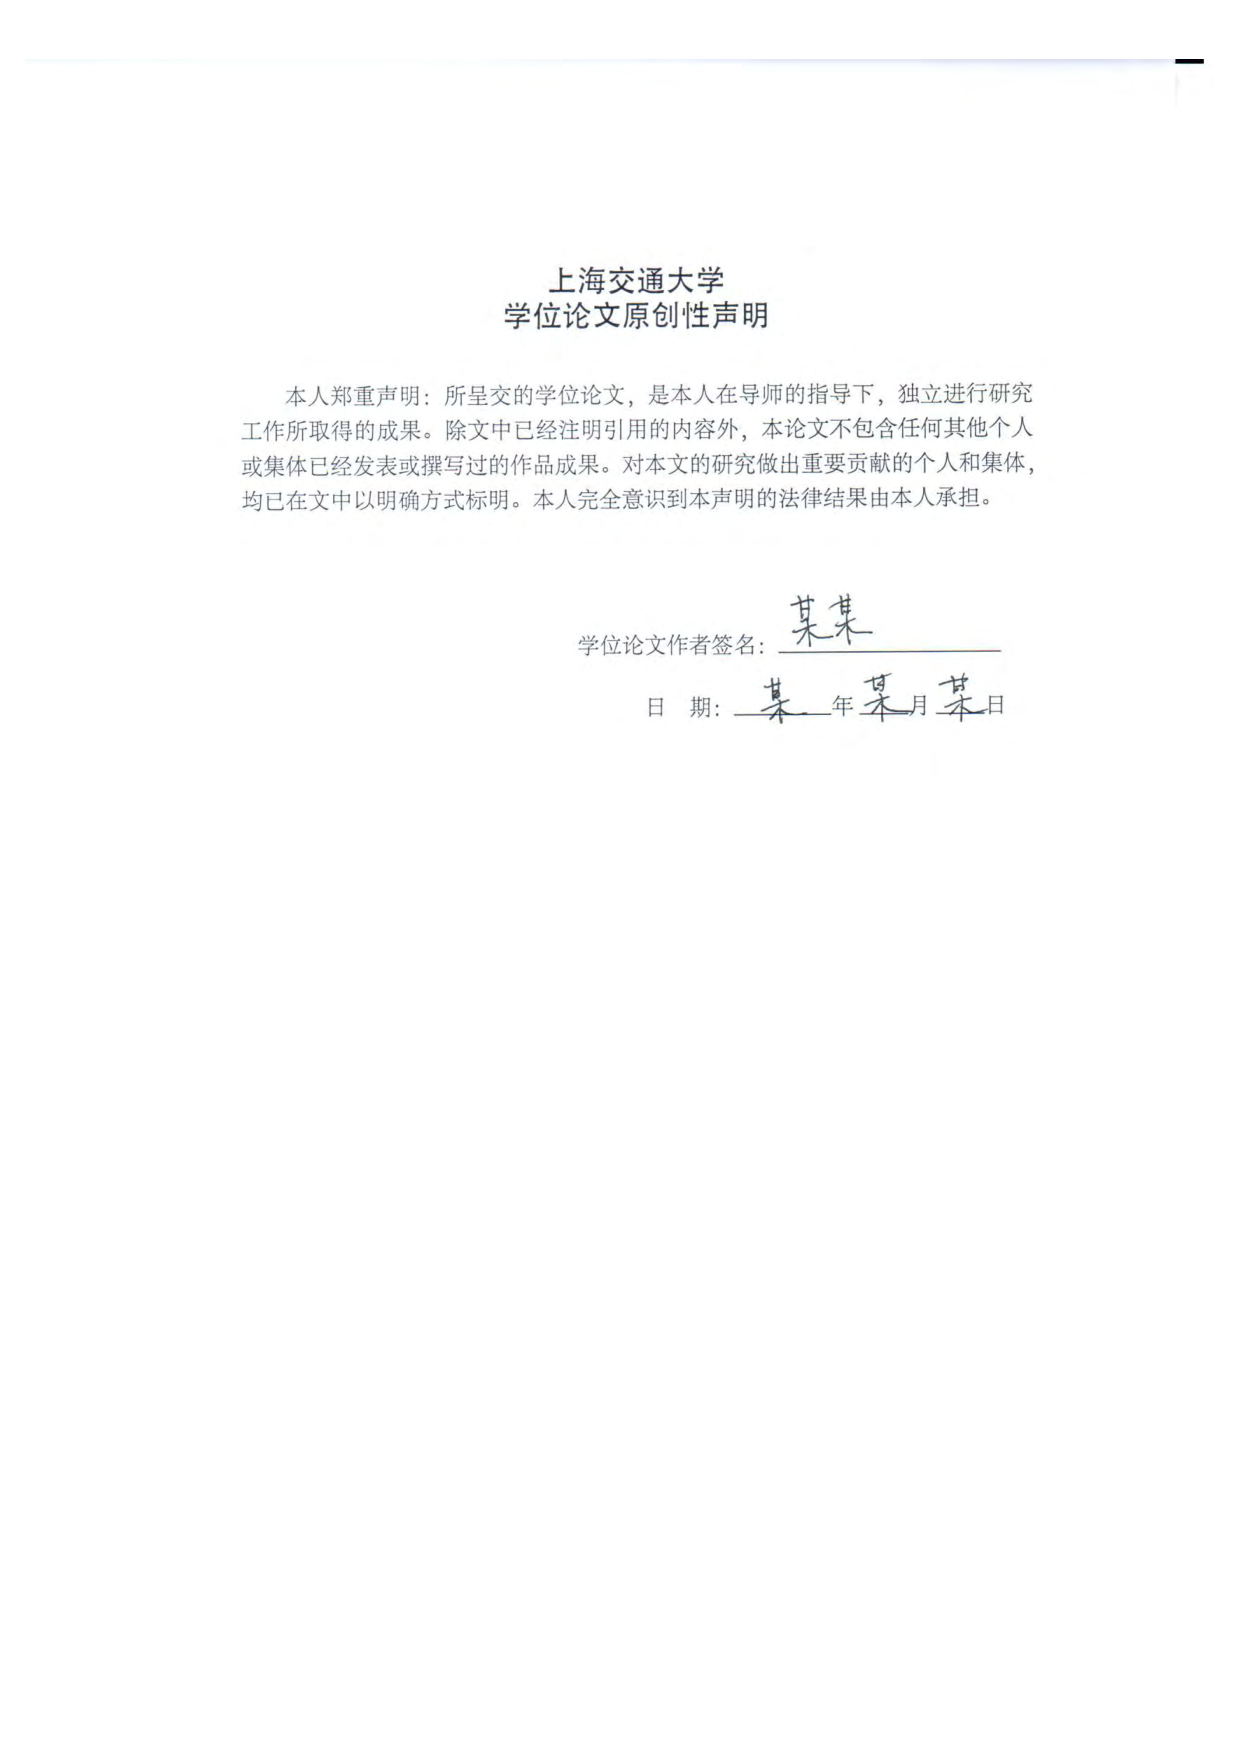
\includepdf{pdf/original.pdf}
  \cleardoublepage
  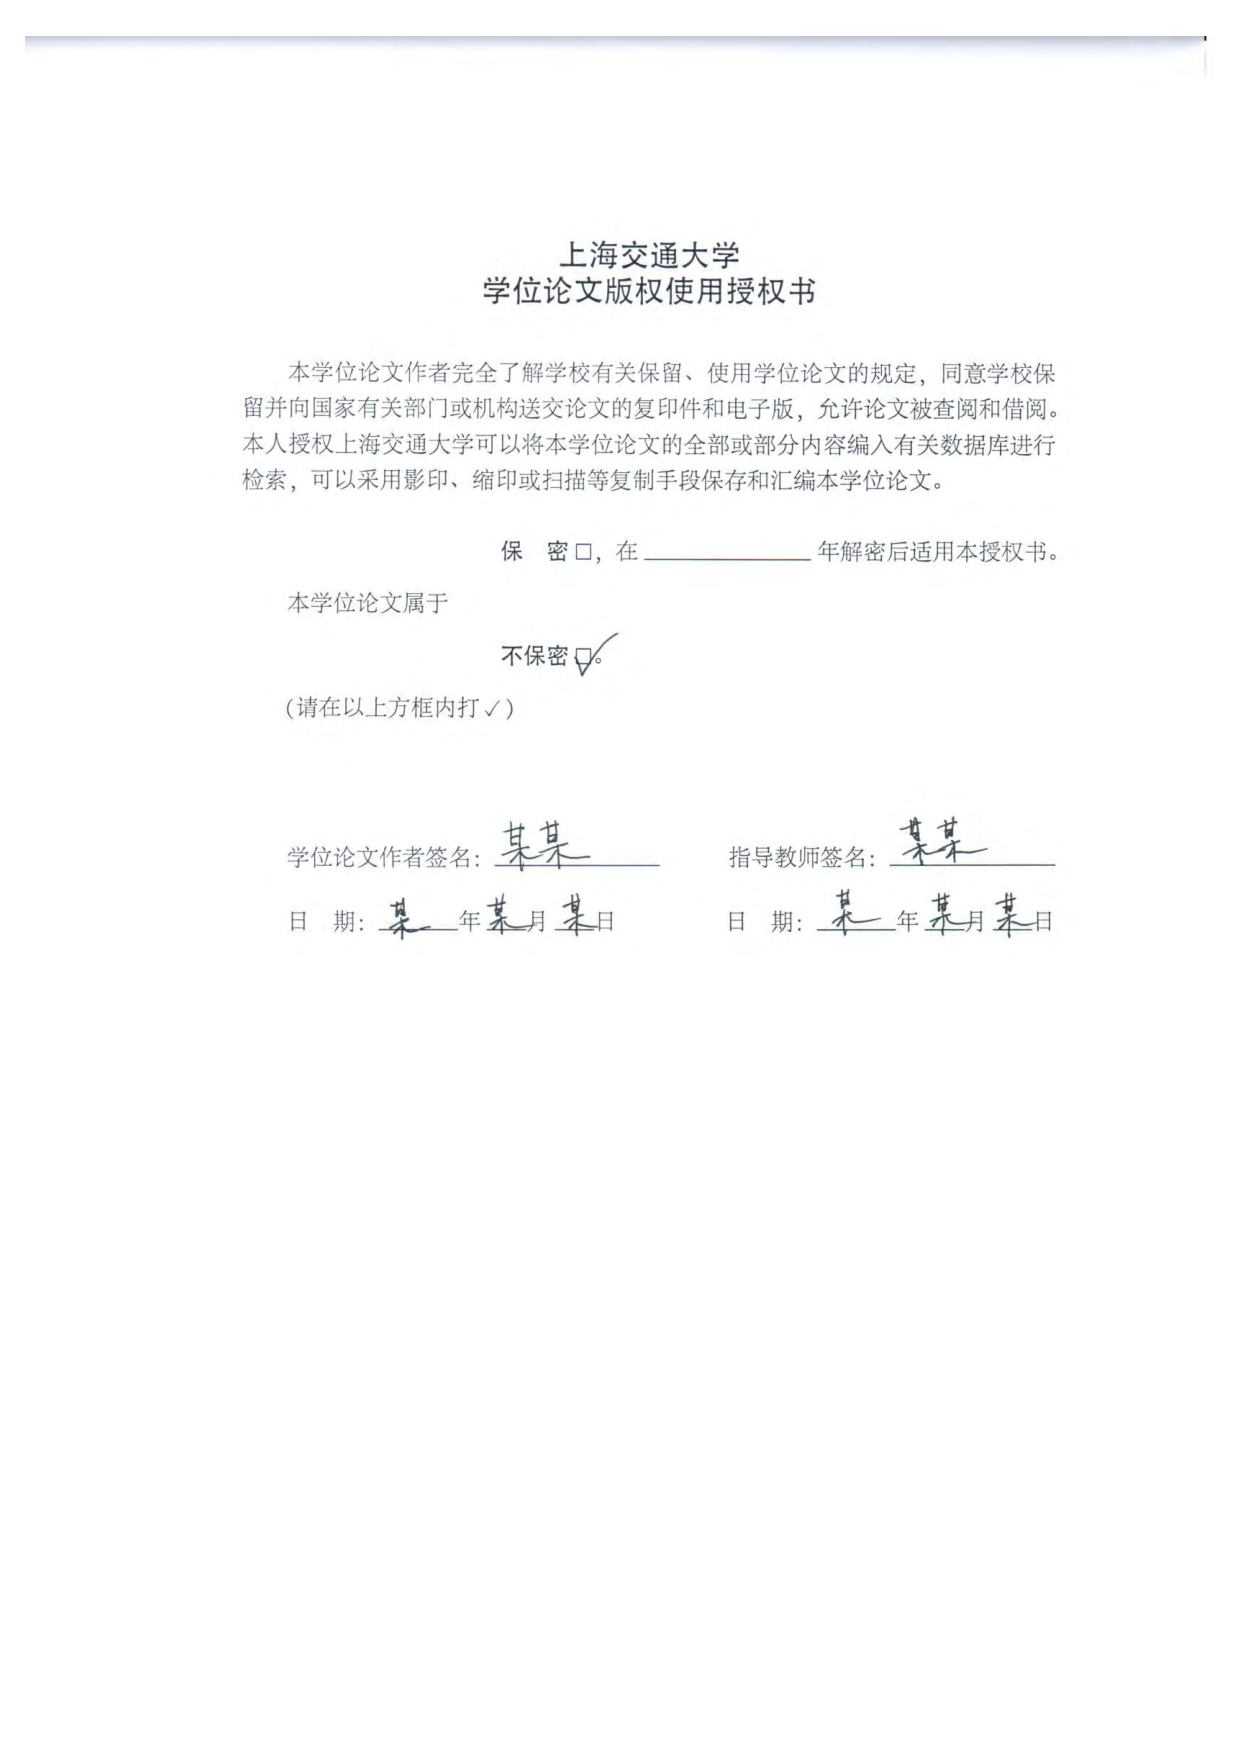
\includepdf{pdf/authorization.pdf}
  \cleardoublepage
\else
\ifsjtu@review\relax
% exclude the original claim and authorization
\else
  \makeDeclareOriginal
  \makeDeclareAuthorization
\fi
\fi
\makeatother

\frontmatter % 使用罗马数字对前言编号

% 摘要
%# -*- coding: utf-8-unix -*-
% !TEX program = xelatex
% !TEX root = ../thesis.tex
% !TEX encoding = UTF-8 Unicode
%%==================================================
%% abstract.tex for SJTU Master Thesis
%%==================================================

\begin{abstract}
  \textbf{第一部分:肠道菌群模式与早产儿坏死性小肠结肠炎和迟发型脓毒血症研究}
    \begin{description}
      \item[目的] 探究早产儿坏死性小肠结肠炎(NEC)和迟发型脓毒血症(LOS)的发生发展与早产儿出生后肠道菌群定植模式的相关性。
      \item[方法] 入组24名早产新生儿,其中4名在住院后发展为NEC,3名为LOS,其余17名为无肠道感染对照组。从出生后的第一天开始收集粪便标本,纵向收集直至患儿出院,共收集192个粪便样本。扩增每个粪便样品的16s rRNA基因的细菌V3~V4区域并测序;后续分析包括:OTU聚类,各分类水平注释,多样性分析和多级物种判别分析。
      \item[结果] 从出生后第14天开始,肠道微生物群定植模式开始在NEC,LOS及其匹配的对照组之间出现差异。迟发型脓毒症早产儿的肠道微生物群多样性最低(Shannon指数= 1.66),对照组保持最多样化(Shannon指数= 0.88,p = 0.01)。潜在致病菌属肠球菌(20.86%)、葡萄球菌(8.67%)和链球菌(8.58\%)的相对丰度在NEC患者中最高(p = 0.034),而在LOS组中为克雷伯氏菌(42.15%,p = 0.023)。对照组较NEC和LOS组含有更多的乳球菌(分别为13.76\%, 7.98\%和3.66\%,p = 0.028)
      \item[结论] 肠道菌群定植失调与早产儿NEC和LOS发生和发展相关,尤其是潜在致病菌属,包括链球菌、葡萄球菌和克雷伯菌的相对丰度增加与上述疾病发展相关。
    \end{description}

  \textbf{第二部分:儿科肠道炎症性疾病与肠道菌群研究}
    \begin{description}
      \item[目的] 比较先天性巨结肠(HD)、先天性巨结肠小肠结肠炎(HAEC)、坏死型小肠结肠炎(NEC)和炎症性肠病(IBD)肠道菌群的异同。
      \item[方法] 入选HAEC患儿4例,HD患儿7例,NEC患儿6例,IBD患儿7例,共24例。采集其横向粪便标本,共58个,其中HAEC标本14个,HD标本22个,NEC标本15个,IBD标本7个。扩增每个粪便样品的16s rRNA基因的细菌V3~V4区域并测序;后续分析包括:OTU聚类,各分类水平注释,多样性分析和多级物种判别分析。
      \item[结果] 三组肠道感染患儿,包括HAEC、NEC和IBD的肠道菌群$\alpha$多样性相仿,且均低于巨结肠患儿;另外,菌群内部组成和丰度($\beta$多样性)在四组患儿间未见显著性差异(PC1 = 32.07\%, PC2 = 24.84\%)。从分类进化角度,肠炎患儿菌群在门水平上的组成大致类似;但具体到属水平则各不相同:HAEC患儿以肠球菌为优势菌属(38.02\%,p = 0.01),总体组成成分与HD类似;IBD患儿各菌属丰度大致相当;NEC患儿肠道菌群构成则较为简单,且以克雷博菌属为主导菌。另外,IBD组可见较高水平的韦荣氏球菌(14\%, p = 0.02),后者与肠道黏膜上皮炎症反映密切相关。
      \item[结论] 肠道微生态失衡包括多样性降低、格兰阴性菌丰度增加,其对于肠道炎症状态的影响具有一定共性,这也可能是三种肠炎有着类似临床表现和病理特征的内在关联因素。
    \end{description}
\end{abstract}

\begin{englishabstract}
  \textbf{Part I. Patterened Intestinal Microbiota in Preterm Necrotizing Enterocolitis and Late-Onset Sepsis}
    \begin{description}
      \item[AIM] To profile postpartum pattern progression of intestinal microbiome in necrotizing enterocolitis and late-onset sepsis in preterm infants, with the aim of understanding their etiologic microbiota profiles from a dynamic perspective.
      \item[METHODS] 24 preterm newborns were enrolled, among whom four subsequently developed NEC, three LOS, and the remaining 17 were healthy controls. Starting from the first stool after birth and continuing till discharge, 192 longitudinal fecal samples were prospectively collected from all patients. Bacterial V3~V4 region of 16s rDNA from each stool sample were amplified and sequenced.
      \item[RESULTS] The postpartum gut microbiota colonization started to diverge among NEC, LOS and their matched control groups, from the second week after birth.  Late-onset sepsis infants held the least diversified gut microbiota (Shannon index=1.66), with the control group held the most diversified one (Shannon index=0.88, p=0.01). The relative abundance of the potential pathogenic genus Enterococcus (20.86\%), Staphylococcus (8.67\%) and Streptococcus (8.58\%) were the highest in NEC patients (p = 0.034), while Klebsiella as the most abundant genus in the LOS group (42.15\%, p = 0.023). The control group contained more Lactococcus than the NEC and LOS groups (13.76\%, 7.98\% and 3.66\%, respectively, p = 0.028)
      \item[CONCLUSIONS] Post partum colonization pattern of gut microbiome might predispose preterm newborns to necrotizing enterocolitis or late-onset sepsis, in which reduced diversity of the whole microbiota community and potentially pathogenic genus could have played an essential role in disease progression. Still, more studies are needed to identify etiological strains, underlying mechanisms and correspondent microbial patterns.
    \end{description}

  \textbf{Part II. Pediatric Enterocolitis in Association with Intestinal Microbiota}
    \begin{description}
      \item[AIM] To compare the similarities and differences of intestinal microbiota in Hirschsprung's disease (HD), Hirschsprung-associated enterocolitis (HAEC), necrotizing enterocolitis (NEC) and inflammatory bowel disease (IBD).
      \item[METHODS] 24 patients were enrolled, among them four were HAEC patients, seven were HD patients, six were NEC patients, and severn were IBD. A total of 58 fecal samples were collected, including 14 HAEC samples, 22 HD samples, 15 NEC samples, and 7 IBD samples. The bacterial V3~V4 region of the 16s rRNA gene from each fecal sample was amplified and sequenced; subsequent analysis included: OTU clustering, annotation of each classification level, diversity analysis and multi-level species discriminant analysis.
      \item[RESULTS] The intestinal microbiota from three groups of enterocolitis are similar in diversity and lower than that of children with HD and healthy children of the same age. In addition, the internal composition and abundance of the microbiome ($\beta$ diversity) are similar among four groups (PC1 = 32.07\%, PC2 = 24.84\%). From the perspective of taxonomic evolution, the compositions of the gut microbiota of children with enteritis are similar at the phylum level; however, on the genus level, compositional differences were observed: \textit{Enterococcus} were dominant among the HAEC patients (38.02\%, p = 0.01), and it is similar to the HD patients; the abundance of each genus from the IBD patients is roughly equal; the components of intestinal microbiota from the NEC cases are relatively simpler, and Klebsiella is the dominant bacteria. In addition, higher levels of Veillonella (14\%, p = 0.02) are seen in the IBD group, which is closely associated with intestinal mucosal epithelial inflammation.
      \item[CONCLUSIONS] Intestinal microecological dysbosis, including reduced diversity and increased abundance of Gram-negative bacteria, might contributes to the certain commonality during the intestinal inflammatory state. This may also be an intrinsic correlative factor of three enteritis with similar clinical manifestations and pathological features.
    \end{description}

\end{englishabstract}


% 目录、插图目录、表格目录
\tableofcontents
\listoffigures
\addcontentsline{toc}{chapter}{\listfigurename}     % 将插图目录加入全文目录
\listoftables
\addcontentsline{toc}{chapter}{\listtablename}      % 将表格目录加入全文目录
\listofalgorithms
\addcontentsline{toc}{chapter}{\listalgorithmname}  % 将算法目录加入全文目录

%# -*- coding: utf-8-unix -*-
% !TEX program = xelatex
% !TEX root = ../thesis.tex
% !TEX encoding = UTF-8 Unicode
\begin{nomenclaturename}
\label{chap:symb}

\begin{table}[htbp]
  \centering
 \begin{tabular}{lcl}
  \toprule
  缩略语 & 英文全称 & 中文全称 \\
  \midrule
 NEC & Necrotizing Enterocolitis & 坏死性小肠结肠炎 \\
 HAEC & Hirchsprung-Associated Enterocolitis & 先天性巨结肠相关性小肠结肠炎 \\
 。。 & 。。 & 。。 \\
  \bottomrule
 \end{tabular}
\end{table}

\end{nomenclaturename}
 % 主要符号、缩略词对照表

\mainmatter % 使用阿拉伯数字对正文编号

% 正文内容
%# -*- coding: utf-8-unix -*-
% !TEX program = xelatex
% !TEX root = ../thesis.tex
% !TEX encoding = UTF-8 Unicode
%%==================================================
%% chap1intro.tex for SJTU Master Thesis
%%==================================================

%\bibliographystyle{sjtu2}%[此处用于每章都生产参考文献]
\chapter{绪论}
\label{chap:introduction}

\section{人体肠道菌群及其早期定植特点}
肠道菌群是指定植于人或其他动物消化道内的微生物群落,人体肠道也是体内最大的免疫器官。作为人体本身和外部环境的主要界面,肠道必须保护其免收有害抗原(如毒素和病原体)的侵害,同时容纳和耐受对自身健康有益的共生细菌——这是一项艰巨的任务,因为细菌病原体和共生菌之间平衡的改变将肠道从健康的肠内稳态(intestinal homeostasis)\cite{collier2005innate}转变为不受控制的炎症状态,这可能导致肠道本身的损伤,也可能干扰其他系统的正常生理功能,从而与多种疾病的发生发展息息相关,包括炎症性肠病(Inflammatory Bowel Disease,IBD)\cite{ni2017gut, yoo2017enteric},II型糖尿病\cite{harsch2018role},自闭症\cite{de2014altered, de2013fecal}等疾病。共生细菌为人类宿主的健康提供诸多保障,包括维持肠内稳态\cite{hooper2001commensal},保护其免受外界伤害\cite{rakoff2004recognition},维护和支持消化功能\cite{guarner2006mechanisms},调节肠道免疫功能\cite{round2009gut,abreu2010toll}等。

长久以来,新生儿肠道被认为是一种无菌环境,但近年的研究证实了胎粪中的微生物群和羊水中的潜在微生物群的相关性\cite{ardissone2014meconium},以及早产儿气道内的不动杆菌属(\textit{Acinetobacter})\cite{lohmann2014airway},这表明肠道微生物的获取可能从胎儿在非无菌宫内条件下就开始了。然而,在重复这些研究结果之前,考虑到非基于培养的测序方法\cite{pennisi2014our}中细菌污染的影响以及取样时羊膜可能不完整,其结果应被谨慎考虑。

在生理条件下的胎儿肠道在出生后迅速开始获得共生微生物群;并且如前所述,该过程甚至可开始于子宫内。微生物群的初始组成来源于胎儿母亲的结肠和阴道菌群,阴道分娩的婴儿可以通过产道获得。这些微生物群包括肠杆菌(\textit{Enterobacteriae}),肠球菌(\textit{Enterococci})和葡萄球菌(\textit{Staphylococci})\cite{backhed2005host}。更多研究表明,菌群通过胎盘转移也可能影响肠道微生物组的发育\cite{aagaard2014placenta}。肠道微生物群的获得大致上是一个有顺序的过程,从杆菌门(\textit{Bacilli}),再到$\gamma$-变形菌门(\textit{Gammaproteobacteria})和梭菌门(\textit{Clostridia}),接着其余菌群的连续定植\cite{la2014patterned}。通过母乳喂养,更多益生元及其他免疫因子被引入肠道,能够后续促进肠道共生菌的生长,进一步发展和改变肠道微生物群,从而有益于婴儿​​\cite{ouwehand2005prebiotics}。与剖宫产和/或配方奶喂养的婴儿相比,纯母乳喂养和通过阴道分娩出生的足月婴儿表现出良好的肠道微生物群组成,双歧杆菌(\textit{Bifidobacteria})数量较多,艰难梭菌(\textit{Clostridium difficile})和大肠杆菌(\textit{Escherichia coli})数量较少\cite{demehri2013hirschsprung}。

\section{儿科肠道炎症性疾病与肠道菌群}
\label{sec:enterocolitis}
在临床实践中,常见的儿科肠道炎症性疾病包括但不限于坏死性小肠结肠炎(Necrotizing Enterocolitis,NEC)、先天性巨结肠相关性小肠结肠炎(Hirchsprung-Associated Enterocolitis )和炎症性肠病(Inflammatory Bowel Disease,IBD);炎症性肠病又包括克罗恩病(Crohn’s Disease,CD)和溃疡性结肠炎(Ulcerative Colitis,UC)。这些疾病严重影响患儿肠道功能,进而严重影响患儿后续生活质量,甚者可危及生命。目前,NEC、HAEC、IBD的发病机制均未明确;既往研究表明,肠道菌群紊乱与上述疾病的发病关系密切。

\subsection{坏死性小肠结肠炎与肠道菌群紊乱}
坏死性小肠结肠炎(NEC)是新生儿最常见的胃肠道急症之一。它是一种以小肠黏膜缺血性坏死为特征的疾病,与重度炎症、肠道产气菌侵袭、产气侵入肠道壁和门静脉系统相关\cite{neu2011necrotizing}。大多数坏死性小肠结肠炎患儿在发病前健康状况、生长情况和喂养情况均良好\cite{hallstrom2006laboratory}。早期最常见症状表现为喂养耐受性突然变化。腹部体征包括腹胀、腹部压痛、喂养残留、呕吐(通常为胆汁)、腹泻、血便、肠内喂养管可见胆汁\cite{walsh1988necrotizing, yu1980improving}。其他非特异体征包括腹壁红斑、痉挛和硬结。非特异性系统性发现包括呼吸暂停、呼吸衰竭,嗜睡,体温不稳定。更严重者可发生由感染性休克引起的低血压,20\%的NEC患儿被诊断有并发的菌血症\cite{kliegman1984necrotizing},严重者可致死。

因已发表研究的诊断和数据收集不一致,故其发病率尚未明确\cite{zani2015scavenger}。在不同地区间的发病率无明显差异:美国一项研究统计表明:在过去25年内NEC的发病率稳定在0.3-2.4例/1000新生儿,且常见于胎龄最小的早产儿中\cite{pickard2009short};来自其他国家(包括加拿大、日本等)的统计研究也得出了类似的发病率结论\cite{kawase2006gastrointestinal}。然而,新生儿胎龄对NEC发病的影响较大——NEC在早产儿中发病率更高,且与出生体重和孕龄呈负相关:出生体重低于1000g的新生儿发病率最高(尽管不同研究显示发病率在4\%~50\%或更高);出生体重介于1501-2000g的新生儿,其NEC发病率急剧下降到3.8个/1000活产新生儿\cite{stoll2015trends}。同样对于胎龄为35-36周的新生儿,其发病率也骤减。尽管总体上存在差异,但来自世界各地的研究数据始终表明,随着胎龄和孕周的降低,NEC发病率增加\cite{backhed2005host,rees2010national,yee2012incidence}。

近年来,尽管NEC的早期识别和积极护理治疗已显著改善其临床结果,但其发病率仍然未降低,特别在早产极低出生体重的婴儿中,其发病率依然居高不下。因而,寻找其病因并相应地采取预防措施显得尤为重要。

坏死性小肠结肠炎发病机制尚未明确,但研究表明它是多因素决定的:促炎细胞极联反映加剧的缺血和/或再灌注损伤可能起了重要作用。动物模型中的大量实验研究结果表明,肠道缺血,免疫功能不成熟和免疫功能障碍的相互作用使得肠道菌群易位穿过肠黏膜屏障,导致炎症介质,包括白三烯,肿瘤坏死因子(Tumor Necrosis Factor,TNF),血小板活化因子(Platelet Activating Factor,PAF)扩散与腔内胆汁酸释放,引发不同程度的肠道损伤,并损伤引发全身受累\cite{good2015breast,miller1990casein}。流行病学调查表明了感染作为因素之一,包括格兰阴性菌、真菌和病毒\cite{de2004early,hodzic2017role,denning2017pathogenesis}。

既往许多动物实验发现,无菌(Germ Free,GF)小鼠模型在出生后不并发NEC\cite{rozenfeld2001role},引入正常小鼠肠道菌群后,肠道内潘氏细胞(Paneth cells)受损伤,肠道上皮细胞(Intetinal Epithelial Cell)的TLR4信号介导增强\cite{white2017paneth}。

近年来临床研究也致力于发现NEC的特定致病菌。有研究表明,与对照组相比,早发型NEC的患儿在发病早期,肠道内厌氧芽孢杆菌丰度增加;而晚发型NEC患儿在发病前6天大肠志贺杆菌(\textit{Escherichia shigella})比例增加,发病前3天,阪崎肠杆菌(\textit{Cronobacter sakazakii})显著升高\cite{zhou2015longitudinal}。美国一项大型前瞻性病例对照研究发现,在混合模型中,NEC的发病与肠道内革兰氏阴性厌氧杆菌 $\gamma$-变形菌(\textit{Gamma-Proteobacteria})的丰度呈正相关,与专性厌氧菌,尤其是厚壁(\textit{Negativicutes})和梭状芽胞杆菌(\textit{Clostridia})丰度呈负相关\cite{la2014patterned}。

\subsection{先天性巨结肠,先天性巨结肠肠炎与肠道菌群紊乱}
先天性巨结肠(Hirschsprung’ s disease,HD)是病变肠段粘膜下和肌间神经丛副交感神经节细胞缺失,导致病变结肠持续痉挛收缩,近端肠管扩张,肠内容物排出受阻为特征的一种先天性肠道动力障碍性疾病。该病是小儿外科常见疾病,占消化道畸形的第二位\cite{langer1999transanal}。HD可以经外科手术切除无神经节细胞的肠管而治愈。然而,有高达40\%的HD患儿在巨结肠根治术后仍可能罹患巨结肠小肠结肠炎(Hirschsprung’s disease associated enterocolitis,HAEC),说明缺乏神经节细胞并非HAEC唯一的病因。HAEC是HD最常见和最严重的并发症,文献报道其发病率为20\%-58\%,复发率达50\%,病死率为1\%-10\%\cite{frykman2012hirschsprung}。

目前HAEC的具体发病机制仍然未明\cite{austin2012pathogenesis}。近年来,有研究显示,由于先天性巨结肠肠道神经系统的紊乱可能增加肠道对特定病原菌感染和定植的敏感性,肠道微生态失衡可能可能是HAEC的主要发病机制\cite{frykman2012hirschsprung}。巨结肠根治术后发作的HAEC的治疗(去除机械性梗阻病因后)包括肠道休息、肠道灌洗、全身抗生素应用等,表明肠道菌群紊乱可能是HAEC起病和复发的启动因素。如何在源头上明确HAEC致病菌,并阻断肠道微生态失衡的恶性循环,可能是防治HAEC的解决之道。

近30年来许多临床和动物研究致力于发现HAEC特定的致病菌,尽管有一些致病菌被认为可能与HAEC发病有关,如艰难梭状芽孢杆菌\cite{thomas1982association},大肠杆菌\cite{thomas1986enterocolitis},轮状病毒\cite{wilson1990microbiological}等,但迄今为止,尚无明确结论,主要原因是受限于依赖细胞培养的技术,以及肠道菌群的复杂性。由于肠道菌群数量庞大,种类繁多,有85\%的肠道细菌无法由培养得到。有学者利用扩增rDNA限制性片段分析技术对一例反复发作HAEC的3岁患儿进行了纵向系列粪便(共15次)检测,发现HAEC发作与特定肠道菌群分布模式有关,并受到应用抗生素的影响\cite{de2010genomics}。

目前国内外应用宏基因组学测序和分析技术研究肠道菌群在HAEC中的作用的研究较少,检索得相关发表文章共4篇,其中2篇是本课题组的临床前期研究\cite{yan2014characterization,li2016characterization}。我们在手术中提取HAEC和HD患儿不同肠道部位的粪便标本,比较其肠道菌群特点。研究中最大的发现是,HAEC和HD患儿肠道菌群种类存在明显差异,而远端无神经节细胞肠道和近端有神经节细胞肠道内样本的肠道菌群种类并无明显差别。这表明,有无神经节细胞并不是影响肠道菌群组成的主要决定因素;而有无特定肠道菌群的定植可能是影响HAEC产生和发展的重要原因。同时,我们也发现,肠道菌群分布也跟患儿的年龄是有一定关系的,不同年龄阶段的患儿肠道微生物菌群差异明显。说明肠道菌群随着患儿年龄的改变有所不同,这也符合从新生儿出生时消化道的无菌状态到2岁时接近成人的总体变化规律。我们进一步研究发现,曾经罹患HAEC患儿在症状缓解期肠道菌群构成依然与发病时的HAEC患儿相似,提示导致HAEC发病的特定肠道菌群分布模式可能持续存在,这也可能是HAEC复发率高达50\%的原因\cite{li2016characterization}。

\subsection{炎症性肠病与肠道菌群紊乱}
尽管儿科IBD的发病机制和诊断程序与成人IBD相似,但是前者的疾病程度较严重,病情进展较快,易发生并发症,易存在生长迟缓,营养不良等。其病因及发病机制尚不完全明确,目前认为遗传易感性、肠道菌群紊乱以及免疫应答异常对于IBD发病起到贡献作用\cite{liang2014role}。

近期,越来越多的研究支持肠道菌群紊乱在IBD发病中的作用。厚壁菌门(\textit{Firmitutes}),尤其是\textit{Firmitutes prausnitzii}在扩罗恩病患者的粪便中丰度减少\cite{mosca2016gut};另外黏附侵袭性大肠杆菌(adherent-invasive \textit{Escherichia coil},AIEC)和副结核分枝杆菌(\textit{Mycobacteriumavium subspecies paratuberculosis})在IBD发病中作用也相对显著。在2012年,AIEC的EC15和EC10菌株被首次发现于IBD患儿肠道炎症组织中\cite{negroni2011characterization};在体外试验中,AIEC在肠道上皮细胞中的复制增值能力很强,可以诱导肿瘤坏死因子TNF-$\alpha$分泌,与克罗恩病患者回肠黏膜病变相关\cite{o2017comparative}。与健康人相比,克罗恩病患儿肠道内真菌紊乱较为明显,表现为担子菌门(\textit{Basidiomycota}):子囊菌门(\textit{Ascomycota})比例降低,以及白色念珠菌(\textit{Candida albicans})丰度增高\cite{sokol2017fungal}。

\section{肠道菌群研究与宏基因组学技术}
宏基因组学技术是指通过直接从样品中提取全部微生物的DNA,构建文库并筛选,利用基因组学的研究策略来研究样品中所包含的全部遗传组成和功能。由于菌群中的大部分微生物尚且被认为“无法培养”,并且传统上认为通过纯培养的方式难以进行微生物进行研究,因此宏基因组方法的出现使研究人员能够通过DNA测序和异源宿主中宏基因组DNA的功能表达,以与培养无关的方式获取和研究这些微生物。宏基因组学揭示了非凡的多样性和新颖性,不仅在微生物群落本身,而且在这些微生物的基因组中。宏基因组分析可涉及基于序列或功能的方法(或两者的组合)。 DNA测序技术的不断改进以及成本的大幅降低使得宏基因组学领域的发展迅速。

宏基因组学方法实现了大量关于人体内微生物群在人类健康和疾病中的研究。例如:利用红基因组测序技术,Belizario等开辟了基于微生物组治疗方法的新领域,包括噬菌体疗法和CRISPR技术的使用,粪菌移植技术(Fecal Microbial Transplantation,FMT)治疗艰难梭菌感染(Clostridia difficile Infection,CDI)等\cite{belizario2015human}。通过宏基组测序分析川崎病(Kawasaki Disease,KD)患者的肠道菌群信息,并揭示了链球菌属丰度增加在其发病急性期所发挥的作用\cite{kinumaki2015characterization}。

基于序列的宏基因组学研究向我们提供了越来越多关于微生物群落组成,结构和功能能力的新认识和新建街。宏基因组学已经成功地用于鉴定许多新的基因,蛋白质和次级代谢物,例如具有工业,生物技术,药物和医学相关性的抗生素。测序技术,表达载体,替代宿主系统和新型筛选试验的未来改进和发展将有助于通过揭示新的分类学和遗传多样性进一步推动该领域。通过研究曾经无法深入探索的和未发现的微生物基因组学、生理学、进化生态学,无疑证明了宏基因组学方法的实用性和可靠性,也说明其将来将揭示从基因到物种的更多的创新和多样发现。

综上,本研究使用Illumina Miseq深度测序平台对NEC、HD和HAEC及IBD患儿的肠道菌群进行测序比对研究,藉以全面深度探索NEC患儿肠道菌群纵向分布特点,并比较NEC,HD,HAEC以及IBD患儿肠道菌群定制模式的差异和相似性,揭示特定菌群定植模式或者致病菌在其四种儿科炎症性疾病发病中以及NEC和HAEC所扮演的角色。另外,本研究对人体肠道菌群研究中取样和保存方法对于研究结果的影响及重要性进行综述。

%# -*- coding: utf-8-unix -*-
% !TEX program = xelatex
% !TEX root = ../thesis.tex
% !TEX encoding = UTF-8 Unicode
%%==================================================
%% chap2nec.tex for SJTU Master Thesis
%%==================================================

%\bibliographystyle{sjtu2}%[此处用于每章都生产参考文献]
\chapter{肠道菌群纵向模式与早产儿坏死性小肠结肠炎研究}
\label{chap:nec}

\section{引言}
肠道菌群紊乱常常见于多种早产并发症,包括坏死性小肠结肠炎(Necrotizing Enterocolitis, NEC)和迟发性败血症(Late-Onset Sepsis,LOS)。前者是一种以小肠黏膜缺血性坏死为特征的疾病,与重度炎症、肠道产气菌侵袭、产气侵入肠道壁和门静脉系统相关\cite{neu2011necrotizing},在早产儿发病率为4~7\%\cite{rees2010national};起病快,进展凶险,严重者可致死。近年来有研究发现肠道菌群紊乱存在于NEC发病期间。后者是一种在出生后72小时后发生的败血症,其是早产儿和极低出生体重的死亡主要原因之一\cite{stoll2002late}。近期,有报道LOS患儿肠道内菌群多样性下降\cite{mai2013distortions},致病菌包括肠球菌(\textit{Enterococcus})丰度增加\cite{stewart2017longitudinal},提示肠道菌群紊乱与LOS发病相关。本研究拟前瞻性观察早产儿出生后总想肠道菌群变化规律,以探究肠道菌群不同变化轨迹与NEC和LOS发生发展的相关规律,为明确其发病机制并早期预防、诊断和治疗提供依据。

\section{材料与方法}
  \subsection{伦理}
  该研究经上海交通大学医学院附属上海儿童医学中心伦理委员会批准(SCMCIRB-K2013022)。 在入组前,取得其监护人理解、同意并于知情同意书上签字。
  \subsection{研究对象}
  于2013年7月至2014年12月间,上海儿童医学中心新生儿重症监护病房(NICU)患儿,
    \subsubsection{入选及排除标准}
      \paragraph{入组标准}
      胎龄小于34周,出生体重不低于950g的早产儿。
      \paragraph{排除标准}
      1)新生儿早发型败血症,2)肝脏疾病,3)肾功能损害(Cr>88μM),4)存在先天肠道发育异常,5)需要进行大型胸部或腹部手术(男性包皮环切术或动脉导管结扎除外),6)预计使用肠外营养(Parental Nutrition, PN)支持供应超过50%的每日热卡摄入量,且时间超过4天,7)静脉注射抗生素(除常规使用头孢噻肟、哌拉西他唑和甲硝唑),8)有口服抗生素史,9)有血便史,10)日龄大于五天者。
  \subsection{诊断标准}
  评估并记录入组患儿一般情况,临床症状体征、实验室检查及影像学检查等,观察其是否发生NEC(II期和III期)或LOS。

  坏死性小肠结肠炎NEC诊断和分级根据“改良Bell分级标准”\cite{bell1978neonatal}:II期,伴有放射性肠扩张,肠梗阻,肠道积气和/或腹部压痛,和/或轻度代谢性酸中毒,肠鸣音减弱,血小板减少症。

  迟发型败血症LOS确诊标准:如果患儿在出生后72小时后,由至少两位新生儿科医生独立检查确认脓毒症体征/症状,血培养或其他体液培养阳性或可疑阳性,并接受过高级别抗生素治疗(例:美罗培南等),则诊断为LOS。

  住院期间无感染性并发症或败血症、无NEC的患儿纳入对照组。

  \subsection{主要实验室试剂及仪器}
  \label{主要实验室试剂及仪器}
    \subsubsection{试剂与材料}
    \begin{enumerate}
      \item PowerSoil\textsuperscript{\textregistered} DNA Isolation Kit:美国MoBio公司
      \item AxyPrepDNA凝胶回收试剂盒: Axygen爱思进生物技术(杭州)公司
      \item TruSeq\textsuperscript{TM} DNA Sample Prep Kit:Illumina中国
      \item 纸质冻存管盒:江苏省中瑞实验器材经营部
      \item 冻存管(规格1.8ml):江苏省中瑞实验器材经营部
      \item 无菌塑料铲子:江苏省中瑞实验器材经营部
      \item 干冰:上海京日实业有限公司
    \end{enumerate}
    \subsubsection{仪器}
    \begin{enumerate}
      \item -80℃实验室冰箱(超低温冰箱):ThemoFisher赛默飞世尔科技(中国)有限公司
      \item 电子天平(型号XSE104):梅特勒-托利多国际贸易(上海)有限公司
      \item 恒温金属浴(型号TU-100C):上海一恒科学仪器有限公司
      \item 小珠研磨器MiniBeatbeater™(型号-16):美国BioSpec实验仪器设备公司。
      \item 台式高速冷冻离心机(型号5427R):Eppendorf艾本德(上海)国际贸易有限公司
      \item 移液器(型号:Eppendorf Reference\textsuperscript{\textregistered} 2;规格:20 μl, 100 μl,200 μl L,1000 μl):Eppendorf艾本德(上海)国际贸易有限公司
      \item 移液器支架系统(The Eppendorf Pipette Holder System):Eppendorf艾本德(上海)国际贸易有限公司
      \item 自封式双层超滤芯吸头(型号Dualfilter T.I.P.S.\textsuperscript{\textregistered} SealMax;规格:20 μl, 100 μl,200 μl,1000 μl):Eppendorf艾本德(上海)国际贸易有限公司
      \item 漩涡混合器(型号:VORTEX-5:江苏省海门市其林贝尔仪器制造有限公司
      \item 2-8℃医用冷藏箱(型号:HYC-940(F)):中国海尔集团
      \item 超微量紫外线分光光度计(型号NanoDrop 2000C):ThemoFisher赛默飞世尔科技(中国)有限公司
      \item PowerPac™ 通用电泳仪电源
      \item 水平小型电泳槽(型号:Sub-Cell\textsuperscript{\textregistered} 96):BIO-RAD伯乐生命医学产品(上海)有限公司
      \item ABI GeneAmp\textsuperscript{\textregistered} PCR仪(型号: 9700):ThemoFisher赛默飞世尔科技(中国)有限公司 美国应用生物系统中国公司
      \item Tanon 4100 全自动数码凝胶图像分析系统:上海天能科技有限公司
      \item QUANTIFLUOR™荧光计仪(型号QUANTIFLUOR™ST/P):Promega - 普洛麦格(北京)生物技术有限公司,上海盛兆生物科技有限公司。
      \item 16sRNA第二代高通量平台(Illumina Miseq):Illumina中国
    \end{enumerate}
  \subsection{粪便标本采集方法}
  \label{粪便标本采集方法}
    \begin{enumerate}
      \item 取得患儿监护人理解、同意并于知情同意书上签字。
      \item 准备无菌手套、干冰(置于密封盒中)、无菌塑料铲子、冻存管。
      \item 患儿排便30分钟内,带手套,使用塑料铲,于尿布附近刮取粪便样本,置于冻存管内,约 1g。
      \item 根据入组患儿编号和采集时间,对样本进行编号后立刻放入干冰盒中,30分钟内储存于-80℃冰箱中备用。
    \end{enumerate}

  \subsection{标本总DNA提取}
  \label{标本总DNA提取}
  本课题使用PowerSoil\textsuperscript{\textregistered} DNA Isolation Kit试剂盒(Catalog No. 12888-100)提取粪便标本总DNA;流程如下所述:
  操作全程都需带手套。
    \begin{enumerate}
      \item 向所提供的PowerBead管中加入不少于0.25克粪便标本(均质化和裂解程序,管内的缓冲剂将(a)帮助分散土壤颗粒,(b)开始溶解腐殖酸(c)保护核酸免于降解)
      \item 使用漩涡混合器,轻轻涡旋混合(开始将样品分散在PowerBead溶液中)。
      \item 检查溶液C1,如果观察到C1沉淀,将溶液置于恒温金属浴60°C直至沉淀物在使用前溶解。溶液C1可以在加热后直接使用。(溶液C1包含SDS和其他裂解细胞所需的阻断成分;SDS作为一种阴离子洗涤剂,也可帮助分解与细菌细胞膜相关的脂肪酸和脂质有关的脂肪酸。金属浴60°C将溶解SDS,但不会损害SDS或其他阻断成分。)
      \item 在PowerBead管中加入60μl溶液C1并手动翻转数次,或也可以短暂涡旋混合。
      \item 使用小珠研磨器MiniBeatbeater™垂直固定PowerBead管,以最大速度涡旋15分钟。(注意:1)标准时间为10分钟,但本课题使用24孔Beatbbeater™,故涡旋时间增加至15分钟;2)涡旋步骤对于完全均质化和细胞裂解是至关重要的。 通过来自步骤1-4的化学试剂和在该步骤引入的机械振荡的组合裂解细胞。 通过在破坏剂存在下随机摇动珠子,珠子与微生物细胞的机械震荡、碰撞将是的微生物细胞完全破裂。)
      \item 确保PowerBead管在离心机中无摩擦、可自由旋转。 在室温下以10,000xg离心1分钟。 (注意:1)转速不应超过10,000 x g,因为管子可能会破裂。2)标准流程离心时间为30秒,由于本课题所收取的样品量有时较多,经尝试,离心时间1分钟的离心效果较好。)
      \item 将第(6)步中收取的上清液转移至干净的2 ml收集管(试剂盒提供)中,该步骤上清液约500μl。
      \item 将250μl溶液C2加入步骤(7)中的收集管中,然后涡旋5秒;在4°C环境中孵育5分钟。(溶液C2为 Inhibitor Removal Technology\textsuperscript{\textregistered}(IRT),含有一种沉淀非DNA有机和无机物质的试剂,包括腐殖质,细胞碎片和蛋白质,同时可去除可能降低DNA纯度并抑制下游DNA应用的污染性有机和无机物质。)
      \item 在室温下,离心步骤(8)中的收集管,转速10,000 x g,离心时间1分钟。
      \item 将步骤(9)中收取的上清液(体积不多于600μl的)转移至新的干净的2 ml收集管(试剂盒提供)中,注意吸头避免碰触沉淀。(此时的沉淀含有非DNA有机和无机物质,包括腐殖酸,细胞碎片和蛋白质。为了获得最佳的DNA产量和质量,请避免转移任何沉淀。)
      \item 将200μl溶液C3加入步骤(10)中的上清液中,并短暂涡旋。在4°C孵育5分钟。(溶液C3为 Inhibitor Removal Technology\textsuperscript{\textregistered},IRT),是另一种沉淀其他非DNA有机和无机物质的试剂,包括腐殖酸,细胞碎片和蛋白质,也可去除可能降低DNA纯度并抑制下游DNA应用的污染性有机和无机物质。
      \item 在室温下,离心步骤(11)中的收集管,转速10,000 x g,离心时间1分钟。
      \item 将步骤(12)中收取的上清液(体积不多于750μl的)转移至新的干净的2 ml收集管(试剂盒提供)中,注意吸头避免碰触沉淀。(此时的沉淀含有非DNA有机和无机物质,包括腐殖酸,细胞碎片和蛋白质。为了获得最佳的DNA产量和质量,请避免转移任何沉淀。)
      \item 使用溶液C4前,将其轻轻摇匀。将1.2ml溶液C4加入步骤(13)中的收集管中(此步骤小心缓慢,避免溶液溢出收集管边缘),然后涡旋5秒。(溶液C4是高浓度盐溶液。 由于DNA在高盐浓度下与二氧化硅紧密结合,因此C4可以调节DNA溶液盐浓度,以使DNA(但可能仍然有低水平的非DNA有机和无机物质)与离心过滤管Spin Filter的滤膜结合。)
      \item 转移675μl步骤(14)中获取的混合液,于离心过滤管Spin Filter中,然后于室温下离心Spin Filter,转速10,000 x g,离心时间1分钟,弃去下层离心液。重复上述步骤,直至步骤(14)中的混合液完全耗尽, 共3次。(此时,高浓度盐溶液中结合DNA,且被选择性结合至Spin Filter二氧化硅过滤膜上。)
      \item 将500μl溶液C5加入Spin Filter中,然后将其于室温下离心,转速10,000 x g,离心时间1分钟。(溶液C5是乙醇基的洗涤溶液,用于进一步清洁与Spin Filter的二氧化硅滤膜结合的DNA。 该洗涤溶液除去残留的盐,腐殖酸和其他污染物,同时使DNA保持与二氧化硅膜结合。)
      \item 弃去步骤(16)中的下层离心液(含有非DNA的无机和有机物质)。
      \item 于室温下,再次将Spin Filter离心,转速10,000 x g,离心时间1分钟。尽可能完全除去残留的溶液C5(乙醇基洗涤溶液),因为乙醇会干扰许多下游DNA步骤,如PCR,限制性消化和凝胶电泳。
      \item 小心将Spin Filter 置于新的干净的2ml收集管(试剂盒已提供)中,避免将任何溶液C5带入新收集管。
      \item 将100μl溶液C6小心加入Spin Filter的白色滤膜上,保证整个滤膜充分浸润超市,然后静置等待1~2分钟。(溶液C6可与滤膜中的高浓度盐溶液结合,促使DNA与盐溶液解离并洗脱。因此,本课题在此处选择将其滤膜于室温下静置等待1~2分钟,以确保DNA更大程度的解离,后续浓度更高而适合建库测序。)
      \item 在室温下,将步骤(20)中的Spin Filter和收集管离心,转速10,000 x g,离心时间1分钟。
      \item 弃去Spin Filter,得到粪便样本总DNA。
      \item DNA提取质控:利用超微量紫外线分光光度计(型号NanoDrop 2000C)检测DNA,目标浓度约50ng/ml。利用1\%琼脂糖凝胶电泳检测DNA提取质量。
      \item 将通过质控的DNA样本置于-80°C冰箱中上海美吉生物医药科技有限公司进行后续扩增。
    \end{enumerate}

  \subsection{总DNA 16s rDNA V3-V4可变区片段的扩增}
  \label{总DNA 16s rDNA V3-V4可变区片段的扩增}
  扩增区域为16 s rDNA V3-V4可变区,合成带有Illumina官方接头序列barcode的特异引物。扩增模版为上述提取的粪便样品总DNA。用338F (5’-ACTCCTACGGGAGGCAGCAG-3’)和806R (5’-GGACTACHVGGGTWTCTAAT-3’) 引物对V3-V4可变区进行PCR扩增,扩增程序为:95℃ 预变性3min,27个循环(95℃ 变性30s,55℃ 退火30s, 72℃ 延伸30s),最后72℃延伸 10min (PCR仪:ABI GeneAmp\textsuperscript{\textregistered} 9700型)。扩增体系为20ul,4ul 5*FastPfu 缓冲液,2ul 2.5mM dNTPs, 0.8ul 引物(5uM), 0.4ulFastPfu 聚合酶;10ng DNA模板。PCR 采用TransGen AP221-02:TransStart Fastpfu DNA Polymerase;PCR仪为ABI GeneAmp\textsuperscript{\textregistered} 9700型。
  扩增质控:为保证后续数据分析的准确性及可靠性,全部样品均按照正式实验条件进行,尽可能使用低循环数扩增,每例样本重复扩增3次,使用2\%琼脂糖凝胶回收PCR产物,利用AxyPrep DNA Gel Extraction Kit (Axygen Biosciences, Union City, CA, USA) 进行纯化,Tris-HCl洗脱,2\%琼脂糖电泳检测。为保证后续数据分析的准确性及可靠性,需满足两个条件,1) 尽可能使用低循环数扩增;2) 保证每个样本扩增的循环数一致。随机选取具有代表性的样本进行预实验,确保在最低循环数中使绝大多数样本能够扩增出浓度合适的产物。
  \subsection{荧光定量}
  \label{荧光定量}
  利用QuantiFluor™-ST (Promega, USA) 进行检测定量。然后根据每例DNA样本的目标测序量,进行相应比例的混合。
  \subsection{Illumina Miseq下一代高通量测序}
  \label{Illumina Miseq下一代高通量测序}
      \subsubsection{文库构建}
      根据Illumina MiSeq 平台 (Illumina, San Diego, USA)标准操作规程将纯化后的扩增片段构建PE 2*300的文库,构建步骤如下:
        \begin{enumerate}
          \item 连接“Y”字形接头;
          \item 使用磁珠筛选去除接头自连片段;
          \item 利用PCR扩增进行文库模板的富集;
          \item 氢氧化钠变性, 产生单链DNA片段,使用试剂TruSeqTM DNA Sample Prep Kit。
        \end{enumerate}
      \subsubsection{高通量测序}
      使用Illumina公司的Miseq PE300平台进行测序(上海美吉生物医药科技有限公司)
        \begin{enumerate}
          \item DNA片段的一端与引物碱基互补,固定在芯片上;
          \item 以DNA片段为模板,芯片上固定的碱基序列为引物进行PCR合成,在芯片上合成目标待测DNA片段;
          \item 变性、退火后,芯片上DNA片段的另一端随机与附近的另外一个引物互补,也被固定住,形成“桥(bridge)”;
          \item PCR扩增,产生DNA簇;
          \item DNA扩增子线性化成为单链。
          \item 加入改造过的DNA聚合酶和带有4种荧光标记的dNTP,每次循环只合成一个碱基;
          \item 用激光扫描反应板表面,读取每条模板序列第一轮反应所聚合上去的核苷酸种类;
          \item 将“荧光基团”和“终止基团”化学切割,恢复3'端粘性,继续聚合第二个核苷酸;
          \item 统计每轮收集到的荧光信号结果,获知模板DNA片段的序列。
        \end{enumerate}

  \subsection{原始数据处理}
  \label{原始数据处理}
  将测序所得的原始数据进行质控、过滤和优化后,进行OTU聚类和分类学水平注释。后续,本课题则基于OTU进行多种多样性指数分析,以及对测序深度的检测;基于分类学信息,在各个分类水平上,分析了样本所在的生物环境进行群落的组成、结构、相对丰度等特征。在上述分析的基础上,可以对多样本的群落组成和系统发育信息进行多元分析和差异显著性检验等一系列深入的统计学和可视化分析。
    \subsubsection{原始数据保存}
    为方便保存和共享各实验室产生的高通量测序数据,NCBI数据心建立了大容量的数据库SRA(Sequence Read Archive,http://www.ncbi.nlm.nih.gov/Traces/sra)来存放共享的原始测序数据。
    本实验的测序数据上传至NCBI数据库中(BioProject序列号:PRJNA470548)。
    \subsubsection{原始数据管理}
    根据序列索引中的barcode区分各个样本的数据,提取所需的数据后以fastq格式保存, PE数据每个样本有fq1和fq2两个文件,里面为测序两端的reads,且按顺序一一对应。

    Fastq(fq)是第二代测序技术中一种展示测序序列碱基质量的文件格式。每条序列read包含4行信息,其中:第一行为文件识别标志,第一行以“@”开头;第二行为具体的碱基序列;第三行为读段名(ID)(第三行中ID可以省略,但“+”不能省略),也可以含有文件识别标志;第四行是第二行中的序列内容每个碱基所对应的测序质量值,必须包含与序列中的字母相同数量的符号。

    如下所示:

    @HWI-ST531R:144:D11RDACXX:4:1101:1212:1946 1:N:0:ATTCCT

    (第一行)


    ATNATGACTCAAGCGCTTCCTCAGTTTAATGAAGCTAACTTCAATGCTGA\\ \qquad GATCGTTGACGACATCGAATGGG

    (第二行)

    + HWI-ST531R:144:D11RDACXX:4:1101:1212:1946 1:N:0:ATTCCT

    (第三行)

    ?A\#AFFDFFHGFFHJJGIJJJIICHIIIIJJGGHIIJJIIJIIJIHGI@FEHIIJBFFHGJJIIH\\ \qquad HHDFFFFDCCCCEDDCDDCDEACC

    (第四行)
    \subsubsection{接质控与优化数据}
    Illumina Miseq二代测序所得到原始数据PE reads序列为双端序列数据,根据序列件的重叠关系,将成对的reads拼接(merge)成一条序列,同时对reads的质量和merge的效果进行质控过滤,根据序列首尾两端的barcode和引物序列区分样品得到有效序列,并校正序列方向,即为优化数据。
    使用软件:Trimmomatic 软件质控,使用FLASH软件进行拼接。
    具体方法及相关参数:
      \begin{enumerate}
        \item 设置50bp的过滤窗口,如果窗口内的平均质量值低于20,从窗口前端位置截去该碱基后端所有序列,之后再去除质控后长度低于50bp的序列;
        \item  根据双段序列数据的正向和反向两条序列重叠关系(overlap)进行拼接(merge),拼接时overlap之间的最大错配率为0.2,长度需大于10bp。去除无法拼接的序列。
        \item 根据序列首尾两端的barcode和引物将序列拆分至每个样本,barcode需精确匹配,引物允许2个碱基的错配,去除存在模糊碱基的序列。
        \item 根据序列首尾两端的barcode和引物区分样品,并调整序列方向,barcode允许的错配数为0,最大引物错配数为2;
      \end{enumerate}
    \subsubsection{OTU聚类}
    在系统发生学或群体遗传学的研究中,为了便于进行分析,将某一个分类单元(例:品系,门,纲,目,属,种、分组等)人为地设置成同一标志,称为操作分类单元(Operational Unit Taxonomy,OTU)。当在科学研究中分析每个样本测序结果中的各水平分类单元的数目信息前,就需要对序列进行归类操作(cluster);通过这种归类操作,按照彼此的相似性将序列分归为许多小组,此时一个小组就是一个OTU。通常情况下,在97\%的相似水平下的OTU 进行生物信息统计分析。

    基于OTU可以进行多种多样性指数分析,基于OTU聚类分析结果,可以对样品生物群落进行多样性分析,并检测测序深度;基于分类学信息,则可以在各个分类水平上,对样本所在的生物环境进行群落的组成、结构、相对丰度等分析。在上述分析的基础上,可以对多样本的群落组成和系统发育信息进行多元分析和差异显著性检验等一系列深入的统计学和可视化分析。

    使用的UPARSE软件(version 7.1) ,根据97\%的相似度对序列进行OTU聚类,并在聚类的过程中去除单序列和嵌合体。
    \subsubsection{分类学分析}
    为了得到每个OUT所对应的物种分类学信息,采用\href{RDP classifier}{http://rdp.cme.msu.edu/}贝叶斯算法对97\%相似水平的OTU代表序列进行分类学分析,并分别在各个分类学水平:

    domain(域),kingdom(界),phylum(门),class(纲),order(目),family(科),genus(属)比对\href{Silva数据库}{http://www.arb-silva.de},统计各样本的群落组成,默认置信度阈值为70\%。

    多级物种判别分析(LEfSe分析,Linear discriminant analysis Effect Size)是一种用于发掘高维度生物标示和揭示基因组特征的软件。包括基因、代谢和分类,用于区别两个或以上生物条件(或是生物类群)。该分析软件先采用non-parametric factorial Kruskao-Wallis sum-rank test检测具有显著丰度差异特征,并找到与丰度有显著性差异的类群。最后,采用线性判别分析(LDA, Linear Discriminant Analysis)来估算每个物种丰度对于差异效果影响的大小。在Cladogram中,不同颜色的节点表示在对应组别中显著富集,且对组间差异存在显著影响的微生物分类群;浅黄色节点表示在不同分组中均无显著差异,或对组间差异无显著影响的微生物类群。

    \subsubsection{多样性分析}
    多样性指数用来表述一个群落的多样性的统计量,在生物学中可以被用来描述某中环境下的生物多样性。多样性指数常备用来估算任何一个群落,每个成员都属于一个独特的群体或者物种。往往,多样指数的估计量存在一定的偏差,因此相似的值之间往往不能直接比较:本课题主要选择两个空间尺度来比较各分组间和样本间的微生物多样型——$\alpha$多样性和$\beta$多样性。

    $\alpha$多样性指数该指数主要关注局部均匀微生物群落的环境中的物种数目,在本课题中,该微生物群落基于特定分组或特定样本。它反映了群落内物种间通过竞争资源或者利用同一种群落环境而产生的共存结果,它可分为物种丰富度指数、物种均匀度指数和物种多样性指数。

    丰富度指数刻画了微生物群落中所含物种的多少,反映了一定空间范围内生物的丰富程度;其常常受制于群落总体包含的微生物数量,忽略了富集种和稀疏种对于群落多样性的贡献,因而常常将丰富度指数和均匀度指数结合使用。物种多样性指数则结合了物种多样性和多度性,本课题使用Shannon-Wienner指数(Shannon-wiener index)和Simpson多样性指数(Simpson’ diversity index)。其中,前者受物种丰富度和均匀度影响,该指数越大,则反映群落多样性越高,均匀度越低;后者反映了优势种在群落中的地位和作用,也成为生态优势度,与其他多样性指数呈负相关。多样性指数越高,生态优势度越小,均匀度指数越高:
      \begin{enumerate}
        \item Shannon-wiener index
          \begin{equation}
            \label{eq:shanon}
            H{'} = -\sum_{i=1}^{R}p_{i}\ln{p_{i}}\footnote{$p_i$属于第i种物种的个体数占群落中总个体数的比例。下同。}
          \end{equation}
        \item Simpson’ diversity index
          \begin{equation}
            \label{eq:simpson}
            D = \sum_{i=1}^{R}p_{i}^2
          \end{equation}
      \end{enumerate}

    $\beta$多样性指数该指数用来表示生物种类对于群落异质性的反映:不仅描述群落内不生物种类的数量,也考虑它们的相似性及其彼此之间的位置。通常$\beta$多样性表示为群落相似性指数或是同一分组内不同样本中生物物种的周转率。不同分组间生物种类的相似性越差,$\beta$生物多样性越高。

    本课题计算unweighed UniFrac distance, weighed UniFrac distance和Bray-Curtis dissimilarity来进行$\beta$多样性分析,其中weighed UniFrac distance将各物种丰度纳入考虑,而unweighed未对物种丰都进行加权处理。基于$\beta$多样性进行PCoA作图使用上述距离文件进行PCoA和PCA作图,每个代表一个样品菌群整体(即群落),而点与和之间的距离代表两个菌群整体(群落)间的序列相似度。

    PCA(Principal Components Analysis)即主成分分析,也称主分量分析或主成分回归分析法,首先利用线性变换,将数据变换到一个新的坐标系统中;然后再利用降维的思想,使任何数据投影的最大方差在第一个坐标(称为第一主成分)上,第二大方差在第二个坐标(第二主成分)上。这种降维的思想首先减少数据集的维数,同时还保持数据集的对方差贡献最大的特征,最终使数据直观呈现在二维坐标系。

    PCoA(Principal Co-ordinates Analysis)分析即主坐标分析,可呈现研究数据相似性或差异性的可视化坐标,是一种非约束性的数据降维分析方法,可用来研究样本群落组成的相似性或相异性。它与PCA类似,通过一系列的特征值和特征向量进行排序后,选择主要排在前几位的特征值,找到距离矩阵中最主要的坐标,产出结果是旋转后的数据矩阵,改变了坐标系统,并未改变样本点之间的相互位置关系。
    两者的区别为PCA是基于样本的相似系数矩阵来寻找主成分,而PCoA是基于距离矩阵(欧式距离以外的其他距离)来寻找主坐标。

  \subsection{统计学方法}
  \label{统计学方法}
    \begin{enumerate}
      \item 使用Kruskal-Wallis H test检验各分类水平下各物种在各组间的分布(相对丰度)是否存在显著性差异;使用Benjaminia and Hochberg法对\textit{p}值进行多重检验矫正。使用Student’s \textit{t}检验检验各分类水平下各物种在两个组之间的分布(相对丰度)是否存在显著性差异;使用Benjaminia and Hochberg法对\textit{p}值进行多重检验矫正。
      \item 使用Student’s t检验评估两组间多样性指数的差异。若p < 0.05 则表示差异有统计学意义。过$\alpha$多样性分析可以得到群落(分组或者单个样本)中物种的丰度、覆盖度和多样性等信息。
      \item 利用Wilcoxon秩和检验,对每一组中的亚组进行两两检验,在具有显著差异物种类中的所有亚种比较是否都趋同于同一分类级别。
    \end{enumerate}

\section{结果}
  \subsection{患者基本情况}
  2013年7月至2014年12月,共有1148名早产儿入院,其中5名在此期间诊断为坏死性小肠结肠炎(NEC);发病率4.4%, 与总体发病率一致{rees2010national}。 在所有早产儿中,有130名符合我们的研究标准,并向其收集了1698份粪便标本。

  本研究最终选择24个充分采样的早产儿,包括4名坏死性小肠结肠炎(NEC)患儿(2个IIA期和2个IIB期),3个迟发型败血症LOS和17个匹配对照(表S1);共收集192个样本,其中NEC标本47个,LOS标本44个,对照组标本101个,并进行16s rRNA 基因测序。

  本研究中, 所有早产儿的平均胎龄为30.5周(28至33周),平均出生体重为1440克(945克至1950克)。 NEC组有3名女婴和1名男婴,LOS组有2名女婴和1名男婴,对照组有9名女婴和8名男婴。所有患儿均通过剖宫产分娩,并以早产儿配方奶喂养。 NEC的平均发病时间为出生后16天(范围:11至19天),确诊为LOS的平均生命日为12天(图\ref{fig:2dol})。三组的人口统计学比较(表\ref{tab:necdemographic})显示,在胎龄,出生体重和性别百分比方面未见显著差异。

  一旦怀疑发生NEC,患儿会立即得到支持性护理和抗生素治疗——支持性护理包括停止肠内喂养、肠道休息,开始全肠外营养(TPN),补液,纠正代谢性酸中毒,肠道休息。在上海儿童医学中心新生儿重症监护病房,用于预防早产儿出生后败血症的抗生素组合为哌拉西林 - 他唑巴坦,头孢噻肟和甲硝唑。分别在治疗28天和15天后,两名NEC患儿情况好转并重新开始肠内喂养。一名婴儿在家人同意终止治疗并拒绝手术干预后死亡(表\ref{tab:2demograph})。

  根据细菌血培养的阳性结果,来自LOS组的一名患儿被诊断出患有肺炎克雷伯菌菌血症,并且给予美罗培南21天;第二名患儿被诊断患有肺炎克雷伯氏菌和铜绿假单胞菌菌血症并给予美罗培南38天。第三名患儿被诊断为肺炎克雷伯菌菌血症、重症肺炎且对头孢噻肟耐药,因此给予美罗培南13天。

  住院前和住院期间所有患者均未接受益生菌处方。

  \begin{table}[!hpb]
    \centering
    \bicaption[NEC, LOS和对照组早产儿一般情况]
      {早产儿患者一般情况\footnotemark[1]}
      {Demographic characteristics of Preterm NEC, LOS and control groups.}
    \label{tab:necdemographic}
    \begin{tabular}{lp{1.8cm}p{1.8cm}p{1.8cm}p{2cm}c}
      \toprule
         & \textbf{NEC (N=3)} & \textbf{LOS (N=4)} & \textbf{Control (N=17)} & \textbf{Statistical Test} & \textit{p value} \\ \midrule
        \textbf{胎龄(周)} & 29(29-30) & 30(29-31) & 31(28-33) & Kruskal-Wallis test & 0.074 \\
        \textbf{出生体重(克)} & 1416.3 (773.4-2149.1) & 1141.7 (633.4-1649.9) & 1527.4 (1391.6-1663.1) & Kruskal-Wallis test & 0.111 \\
        \textbf{性别} &  &  &  & Fisher's exact test & 0.82 \\
        \multicolumn{1}{r}{女} & 3(75\%) & 2(67\%) & 9(53\%) &  & \\
        \multicolumn{1}{r}{男} & 1(25\%) & 1(33\%) & 8(47\%) &  & \\
        \textbf{诊断时年龄(天)} & 16(11-19) & 16(10-22) & — & Wilcoxon rank-sum test & 0.629 \\
        \textbf{住院时长(天)} & 54.3 (13.5-95.0) & 60.0 (24.8-95.2) & 32.9 (26.3-39.5) & Kruskal-Wallis test & 0.046 \\
        \textbf{标本总数} & 46 & 42 & 103 & — & — \\ \bottomrule
    \end{tabular}
  \end{table}
  \footnotetext[1]{NEC、LOS和对照组在入院时,胎龄、出生体重、年龄和性别无统计学差异。三组住院时常具有显著性差异(p = 0.046),这符合我们的预期,因为NEC和LOS患儿往往需要更长时间恢复,因此住院时间相对更长;比较NEC和LOS组住院时长未见明显统计学差异。胎龄=平均值(下限-下限),出生体重=平均值(95\%置信区间),诊断时年龄=平均值(下限-下限),性别=人数(占本组的百分比),住院时长=平均值(95\%置信区间)
  }

  \subsection{样本及测序信息}
  入选NEC患儿4例,LOS患儿3例, 对照组患儿17例。采集其纵向粪便标本,共192个,其中NEC标本47个,LOS标本44个,对照组标本101个。其他临床资料见表\ref{tab:necdemographic}。

  使用Illumina MiSeq高通量测序、优化后,得到7,472,400条16s rRNA基因序列,碱基数目共3348030799;优化碱基数目为3348,030,799,优化平均序列长度为448bp。
  \subsection{分类学分析}
  对于测序数据进行OTU聚类,采用RDP classifier贝叶斯算法对97\%相似水平的OTU代表序列进行分类学分析,并分别在各个分类水平(从域(domain)到属(genus))统计各样本的群落组成,比对silva数据库得出各群落数量。
    \subsubsection{门(phylum)水平}
    在门水平,三组患儿肠道内以变形菌门(\textit{Proteobacteria})、厚壁菌门(\textit{Firmicutes})、和放线菌门为主导({\textit{Actinobacteria})。变形菌门的丰度在LOS组最高(59.67\%),对照组次之(59.67\%),NEC组最低(38.53\%),三组丰度显著不同(p = 0.017);厚壁菌门(\textit{Bacilli})丰度在NEC组最高(59.59\%),对照组次之(44.88\%),LOS组最低(39.54\%),且三组间丰度呈显著性差异(p = 0.017);放线菌门({\textit{Actinobacteria})的丰度对照组最高(3.40\%),NEC组次之(1.10\%),LOS组最低(0.06\%),三组丰度组间差异显著(p = 0.001)(图\ref{fig:2phylum})。
      %门水平配图
      \begin{figure}[!htp]
        \centering
        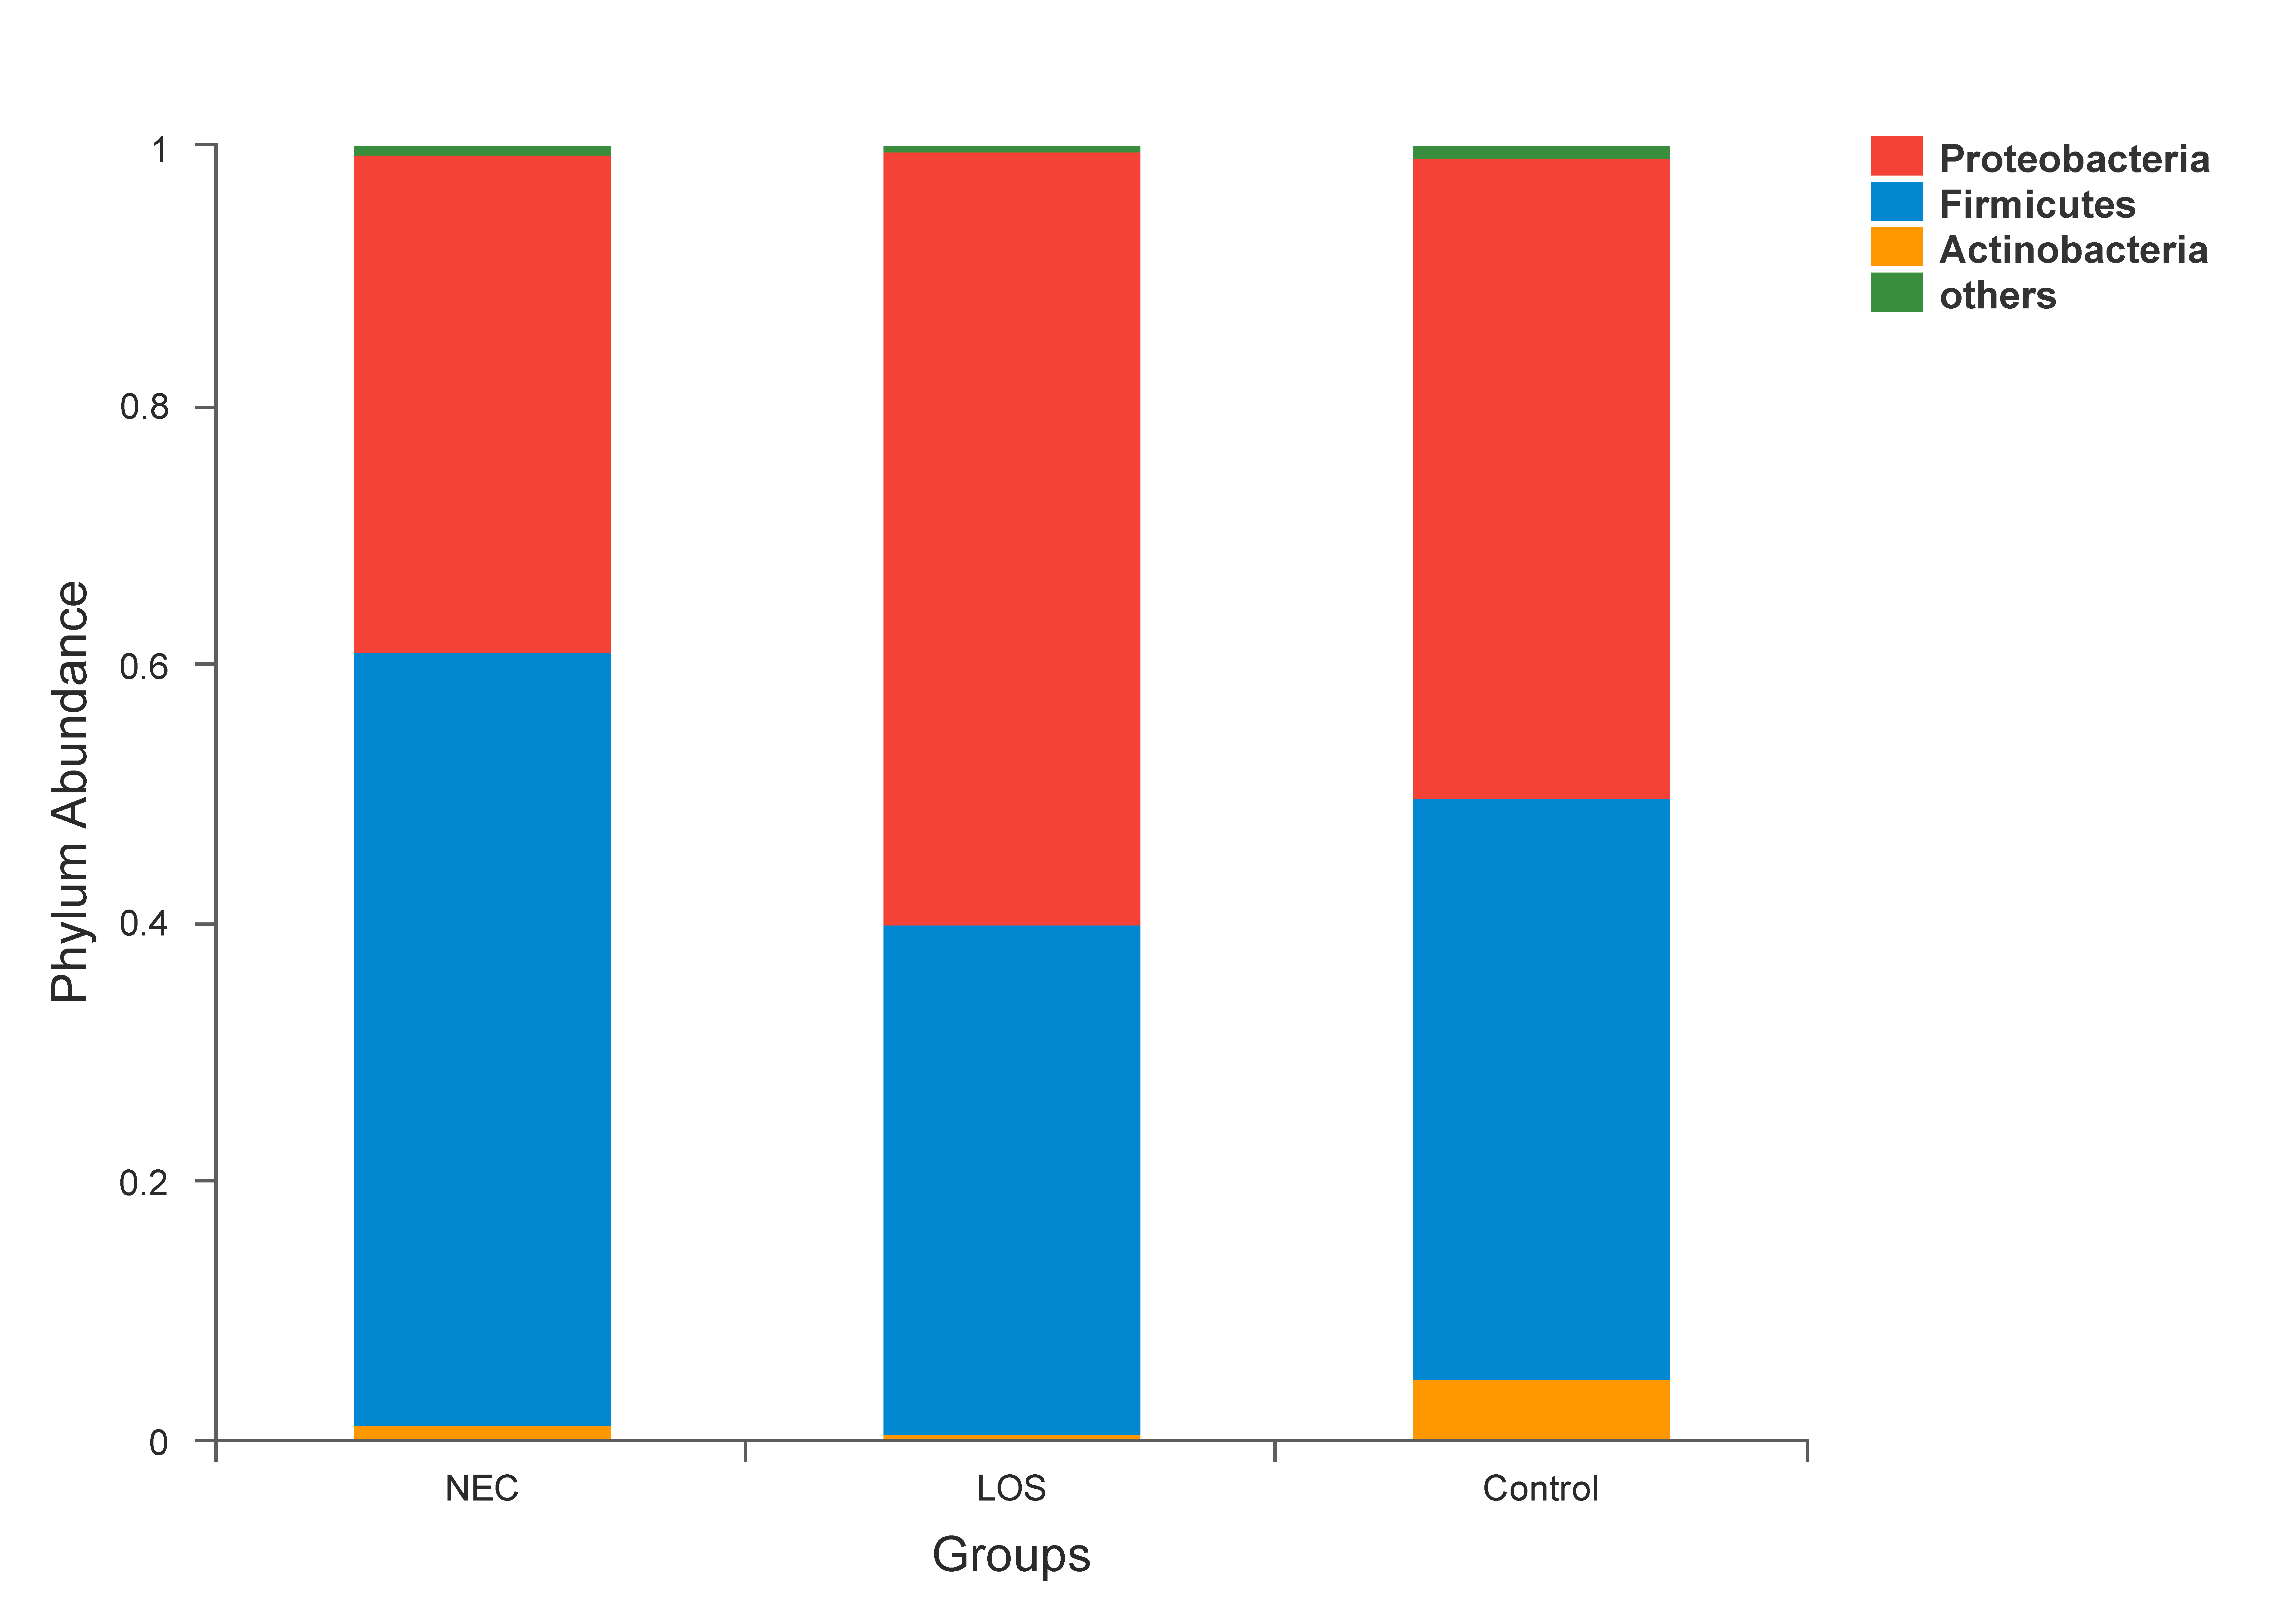
\includegraphics[width=15cm]{2phylum.pdf}
        \bicaption[门水平上NEC, LOS和对照组患儿菌群相对丰度]
          {门水平上NEC, LOS和对照组患儿菌群相对丰度。}
          {Relative Abundance of Phylum in Intestinal Microbiota.}
        \label{fig:2phylum}
      \end{figure}

    \subsubsection{纲(class)水平}
    在纲水平,三组患儿肠道内以$\gamma$-变形菌纲(\textit{$\gamma$-Proteobacteria})、杆菌纲(\textit{Bacilli})、梭菌纲(\textit{Clostridia})和放线菌纲(\textit{Actinobacteria})为主导。$\gamma$-变形菌纲的丰度在LOS组最高(59.57\%),对照组次之(50.51\%),NEC组最低(38.06\%),三组丰度显著不同(p = 0.013);厚壁菌门(\textit{Bacilli})丰度在组最高NEC(53.56\%),对照组次之(39.19\%),LOS组最低(32.17\%),且三组间丰度呈显著性差异(p = 0.015);梭菌纲(\textit{Clostridia})丰度在LOS组最高(6.54\%),NEC组次之(5.36\%),对照组最低(4.86\%),三组丰度差异在统计学上不显著(p = 0.236);放线菌纲(\textit{Clostridia})的丰度在对照组最高(3.40\%),在LOS和NEC丰度相似(前者0.63\%,后者1.01\%,组间差异不显著(p = 0.76)),三组间丰度差异显著(p = 0.001)(图\ref{fig:2class})(图\ref{fig:2class})。
      %纲水平配图
      \begin{figure}[!htp]
        \centering
        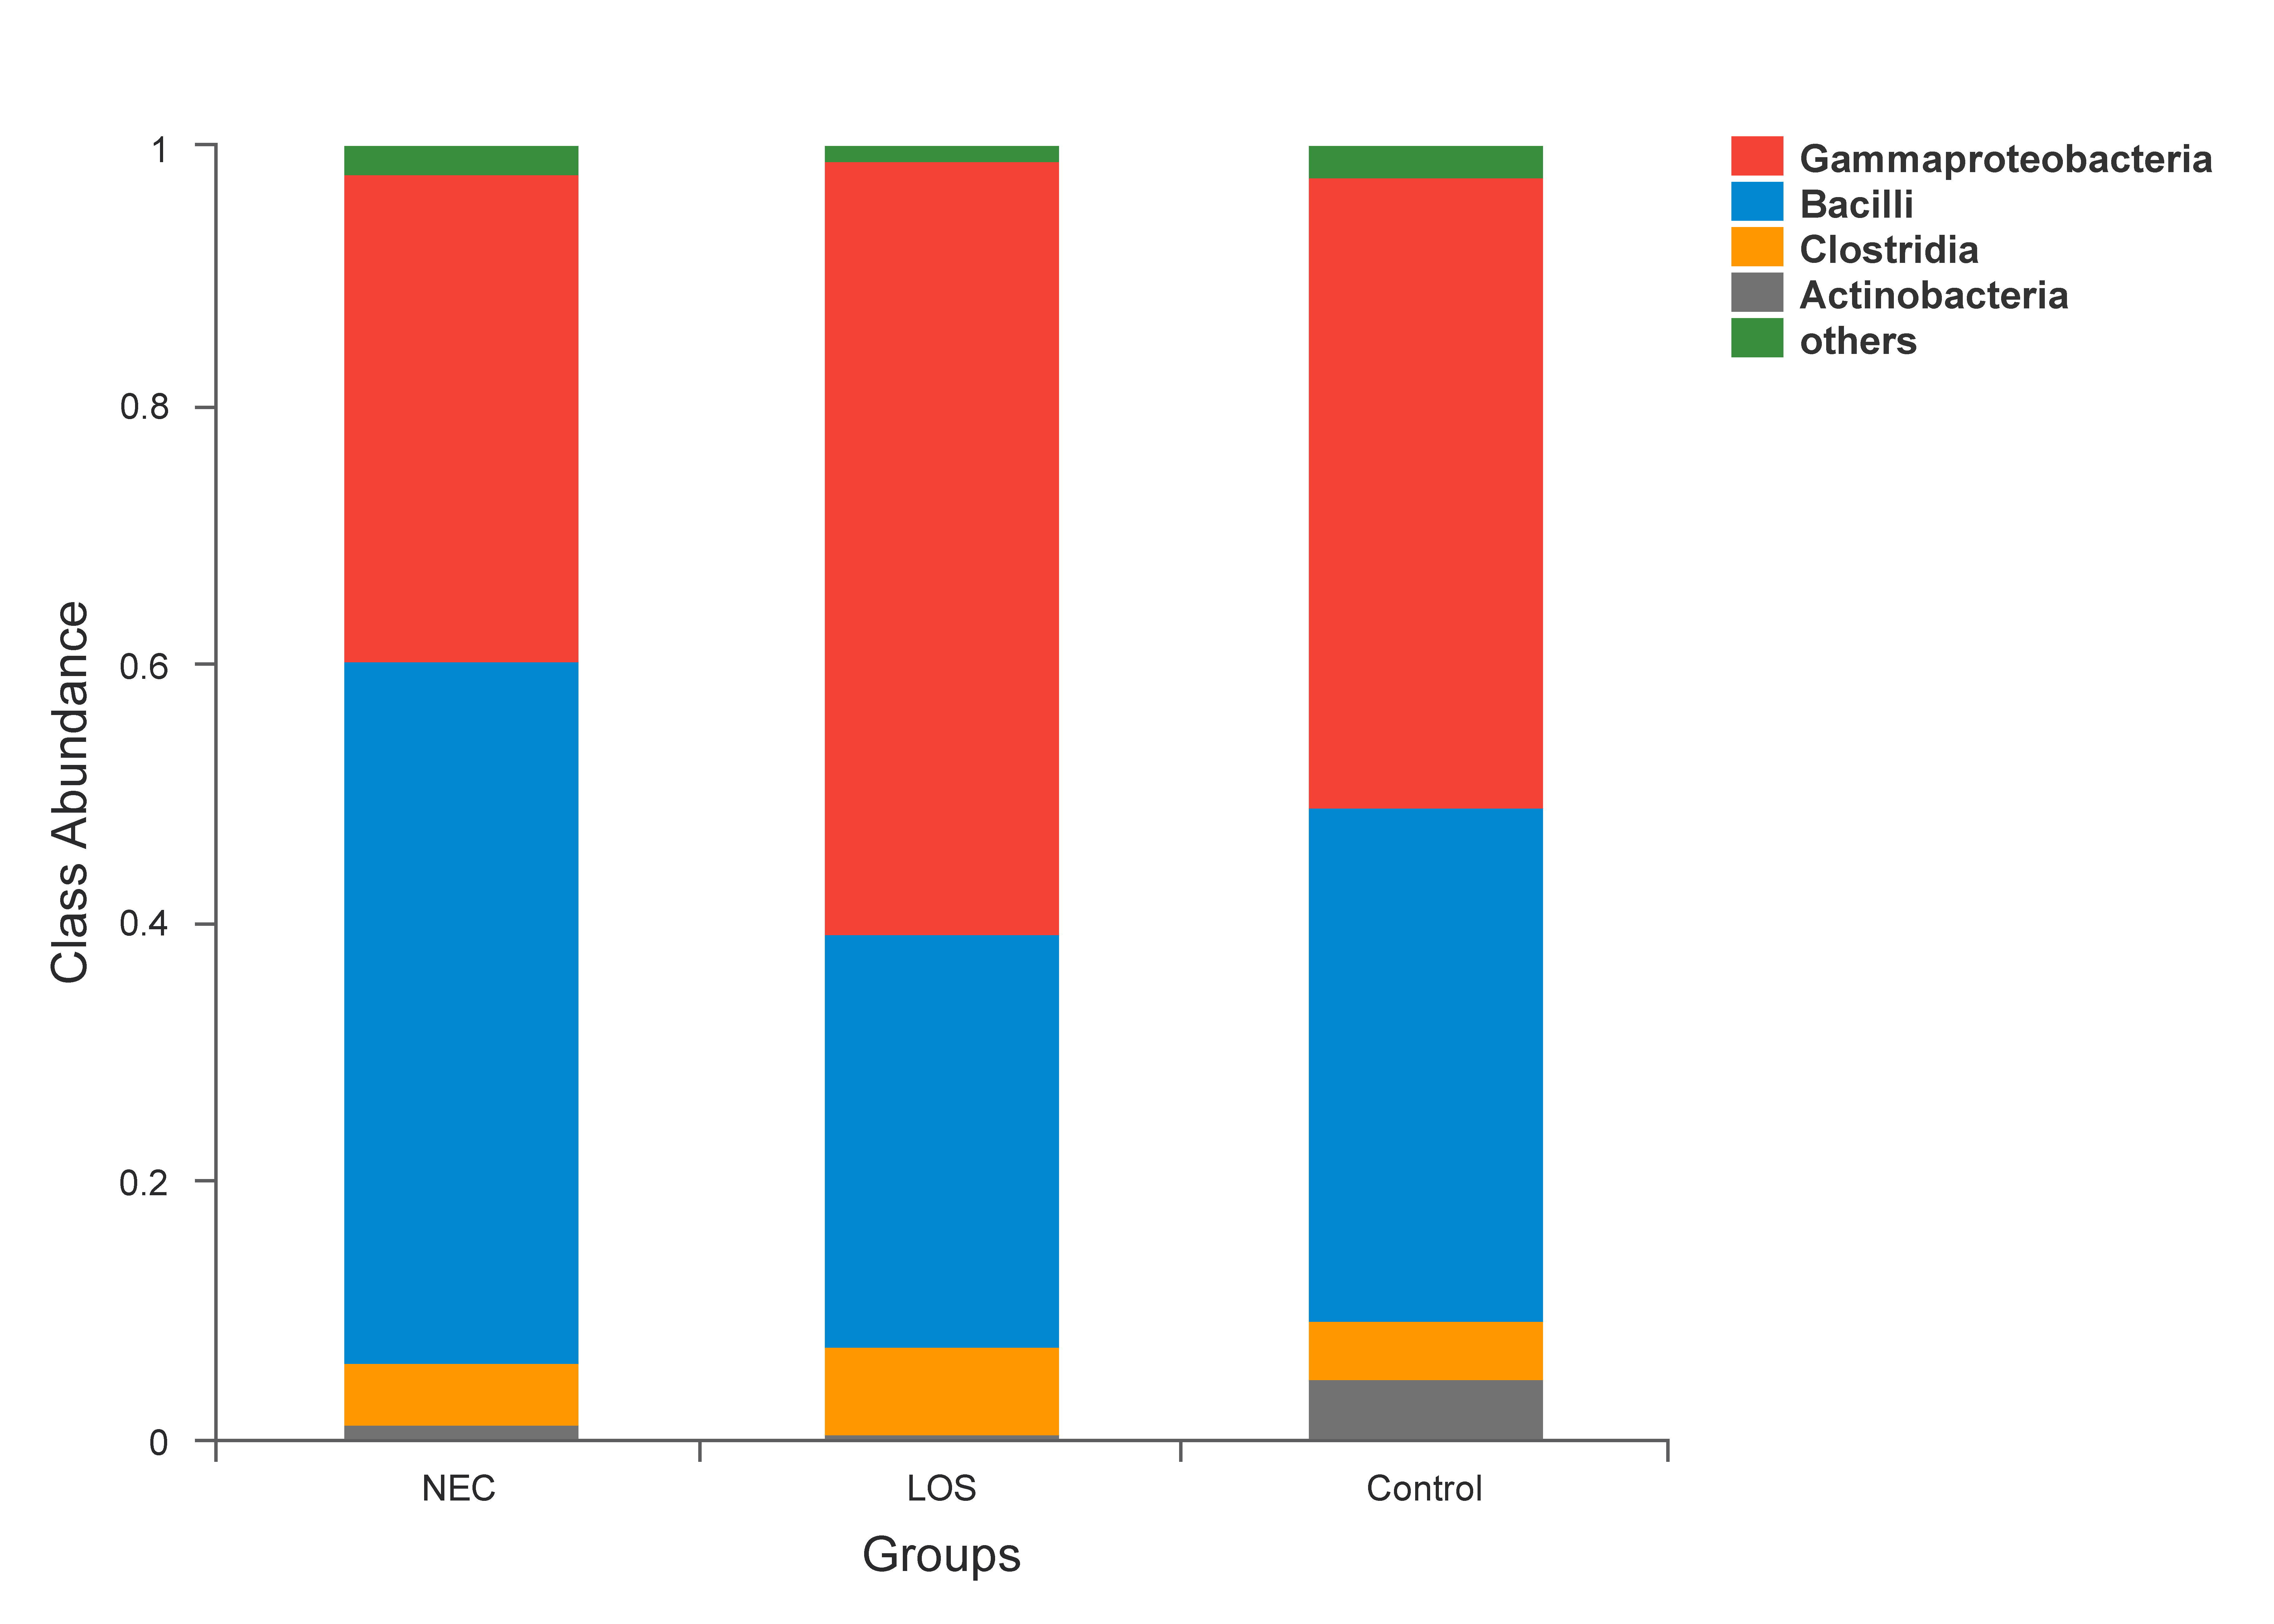
\includegraphics[width=15cm]{2class.pdf}
        \bicaption[纲水平上NEC, LOS和对照组患儿菌群相对丰度]
          {纲水平上NEC, LOS和对照组患儿菌群相对丰度。}
          {Relative Abundance of Class in Intestinal Microbiota.}
        \label{fig:2class}
      \end{figure}

    \subsubsection{目(order)水平}
    在目水平,三组患儿肠道内以肠杆菌目(\textit{Enterobacteriales})、乳杆菌目(\textit{Lactobacillales})、芽孢杆菌目(\textit{Bacillales})、梭菌目(\textit{Clostridiales})、假单胞菌目(\textit{Pseudomonadales})、微球菌目\textit{Micrococcales}为主。肠杆菌目在LOS组最高(57.05\%),对照组次之(40.89\%),NEC组最低(34.87\%),三组丰度差异在统计学上显著(p = 0.011);乳杆菌目在NEC组丰度最高,为37.94\%,在LOS和对照组丰度分别为(27.1\%)和(28.28\%),且三组间乳杆菌丰度差异不显著(p = 0.176);芽孢杆菌目在LOS组丰度(5.08\%)显著低于NEC组(15.62\%,两组比较p = 0.05),对照组丰度为10.91\%;梭菌目分别在三组的丰度类似:NEC组为\%5.36,LOS组为\%6.54,对照组为4.86\%;假单胞菌目在对照组的丰度(8.62\%)显著高于NEC组(3.15\%,p = 0.015)和LOS组(\%2.39,p = 0.015)。另外,棒状杆菌目(\textit{corynebacteriales})和黄色单胞菌目(\textit{Xanthomonadales})为对照组所独有(丰度分别为1.62\%和0.88\%)的菌目(图\ref{fig:2order})。
      %目水平图
      \begin{figure}[!htp]
        \centering
        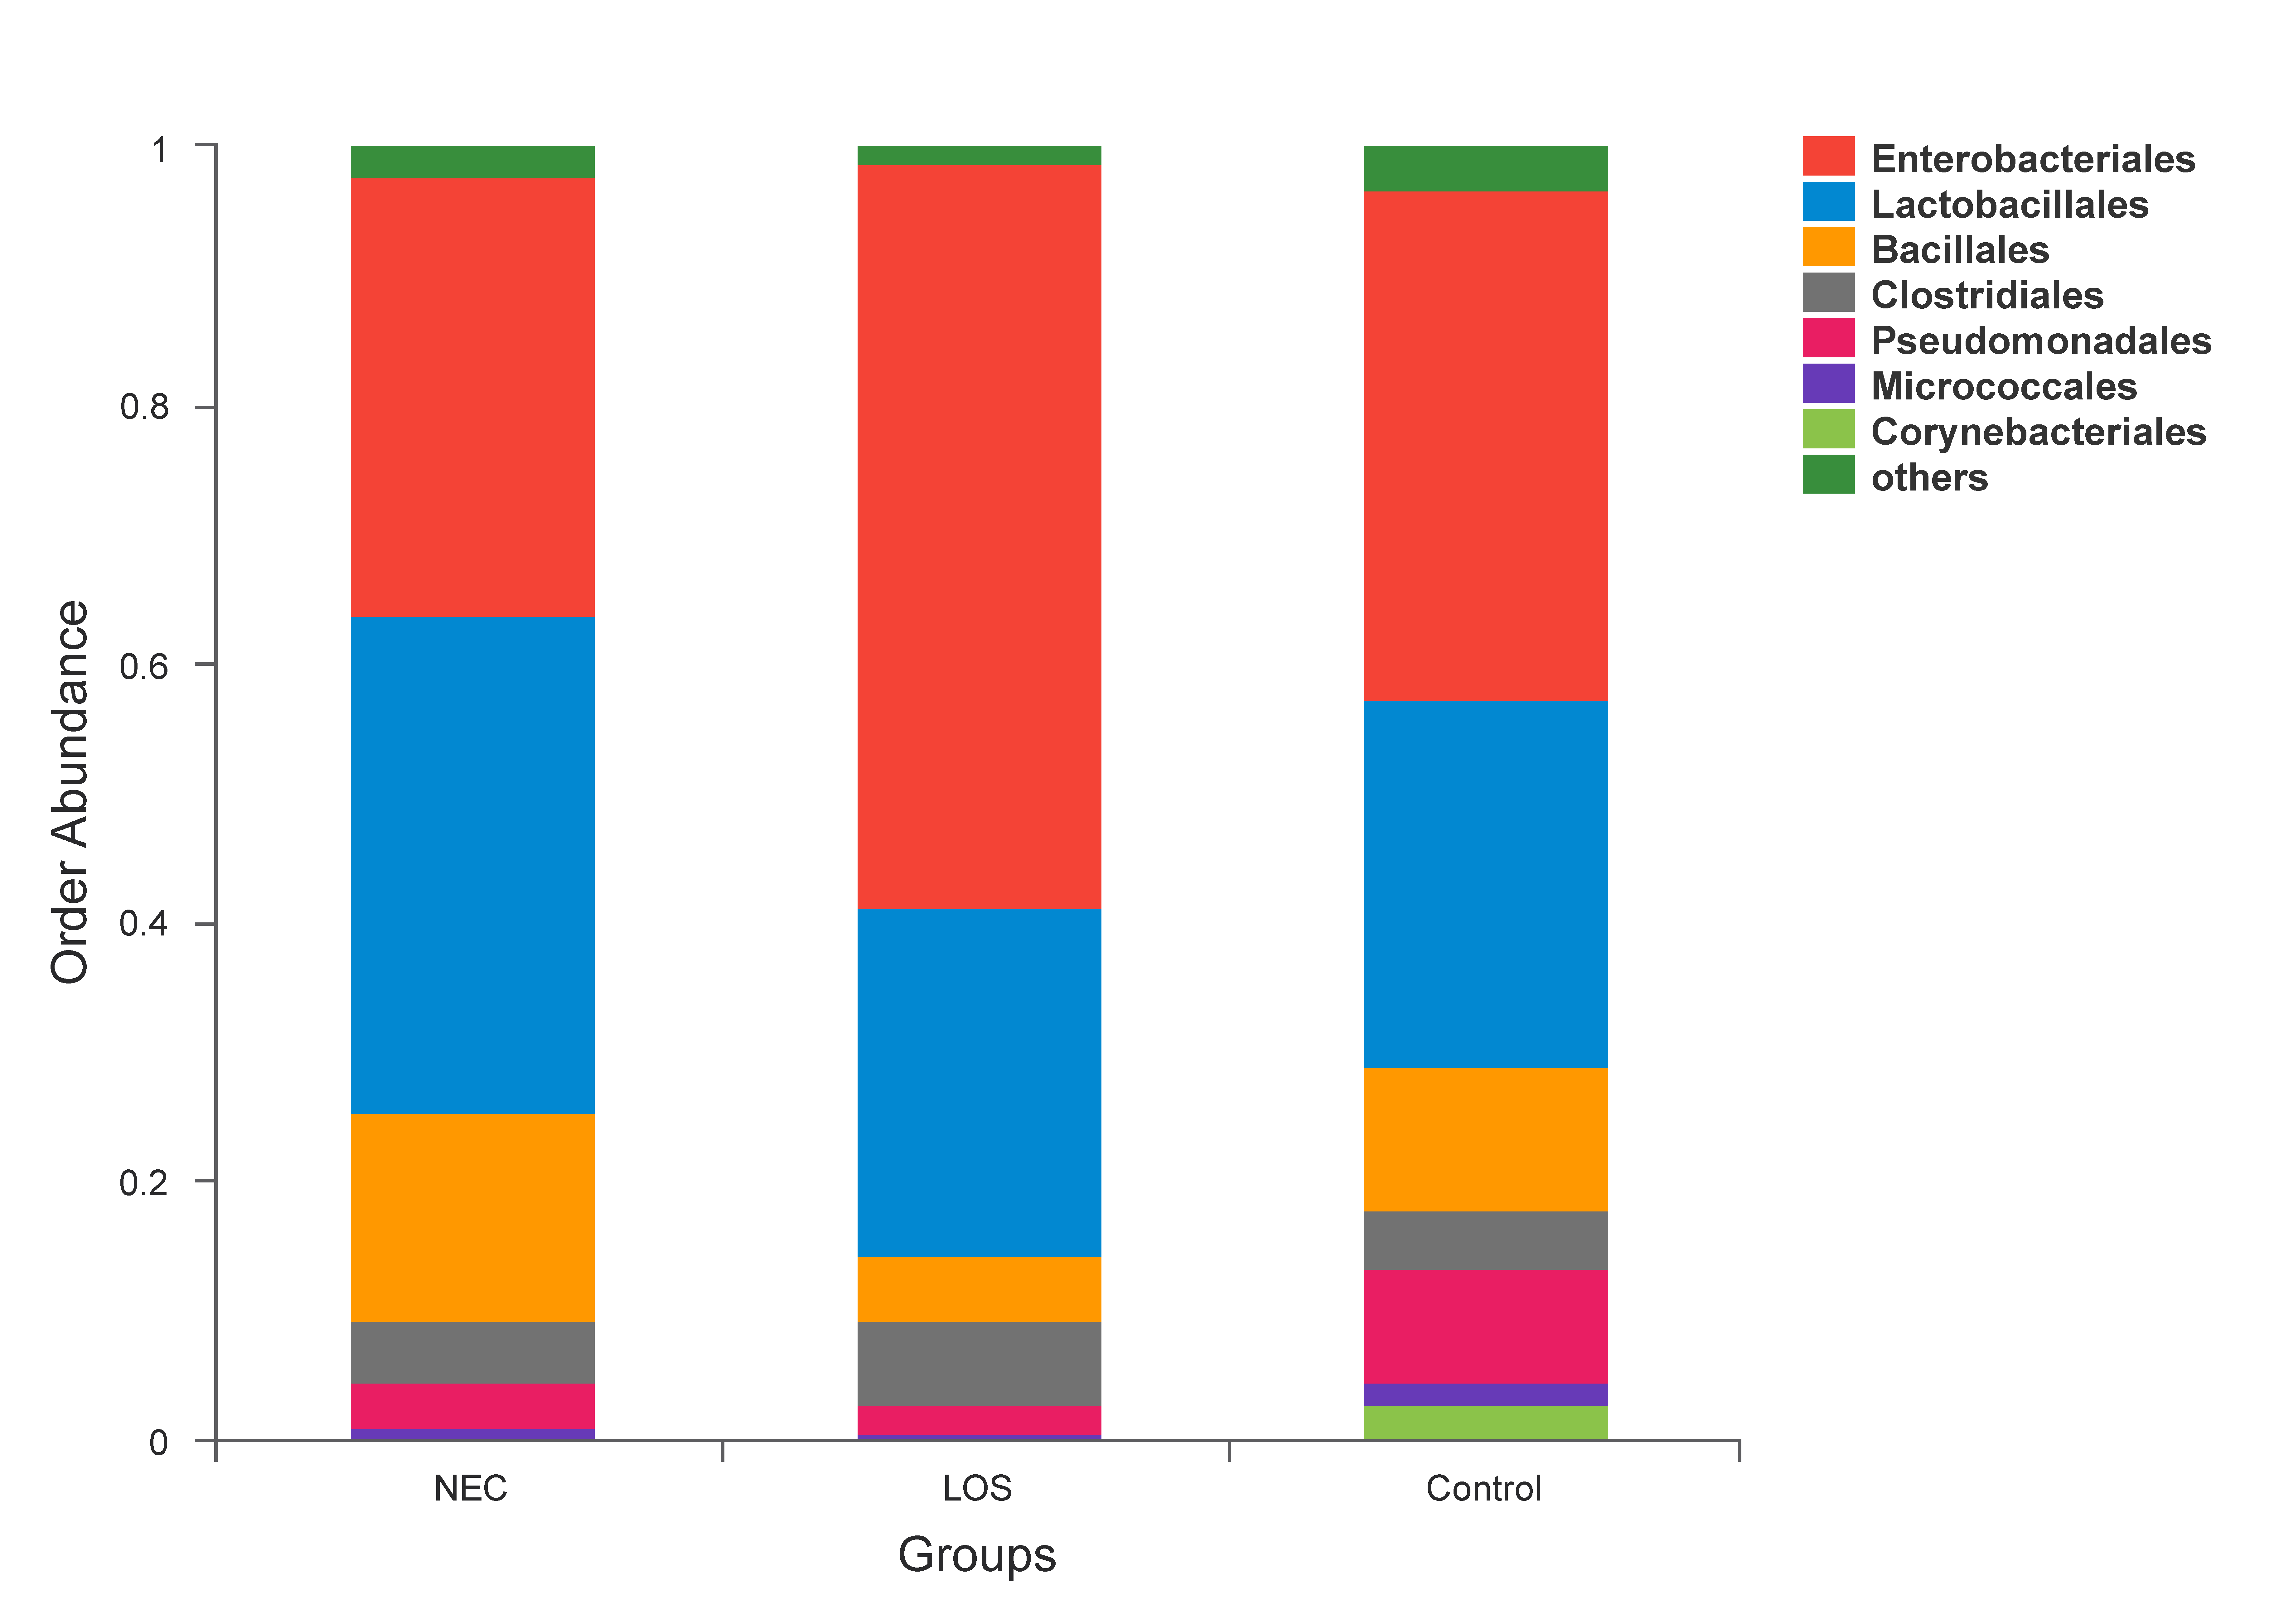
\includegraphics[width=15cm]{2order.pdf}
        \bicaption[目水平上NEC, LOS和对照组患儿菌群相对丰度]
          {目水平上NEC, LOS和对照组患儿菌群相对丰度。}
          {Relative Abundance of Order in Intestinal Microbiota.}
        \label{fig:2order}
      \end{figure}

    \subsubsection{科(family)水平}
    在科水平,三组患儿肠道内以肠杆菌科(\textit{Enterobacteriaceae})、肠球菌科(\textit{Enterococcaceae})、乳杆菌目(\textit{Lactobacillales})、链球菌科(\textit{Streptococcaceae})、葡萄球菌科(\textit{Staphylococcaceae})、假单胞菌科\textit{Pseudomonadaceae}占主导。肠杆菌科丰度在LOS组最高,为57.05\%,NEC组和对照组丰度分别为34.87\%和40.89\%,三组间丰度差异显著(p = 0.011);肠球菌科在三组的丰度分别为NEC组20.86\%,LOS组18.15\%,对照组8.46\%,三组间差异不显著(p = 0.109);LOS组链球菌科百分比(8.70\%)显著低于NEC组(16.67\%,p = 0.)和对照组(19.07\%p = 0.023),NEC组(16.67\%,且三组比较差异不显著(p = 0.438);假单胞菌在三组的丰度分别为NEC组2.41\%,LOS组2.05\%,对照组5.40\%,三组间差异显著(p = 0.039)(图\ref{fig:2family})。
      %科水平图
      \begin{figure}[!htp]
        \centering
        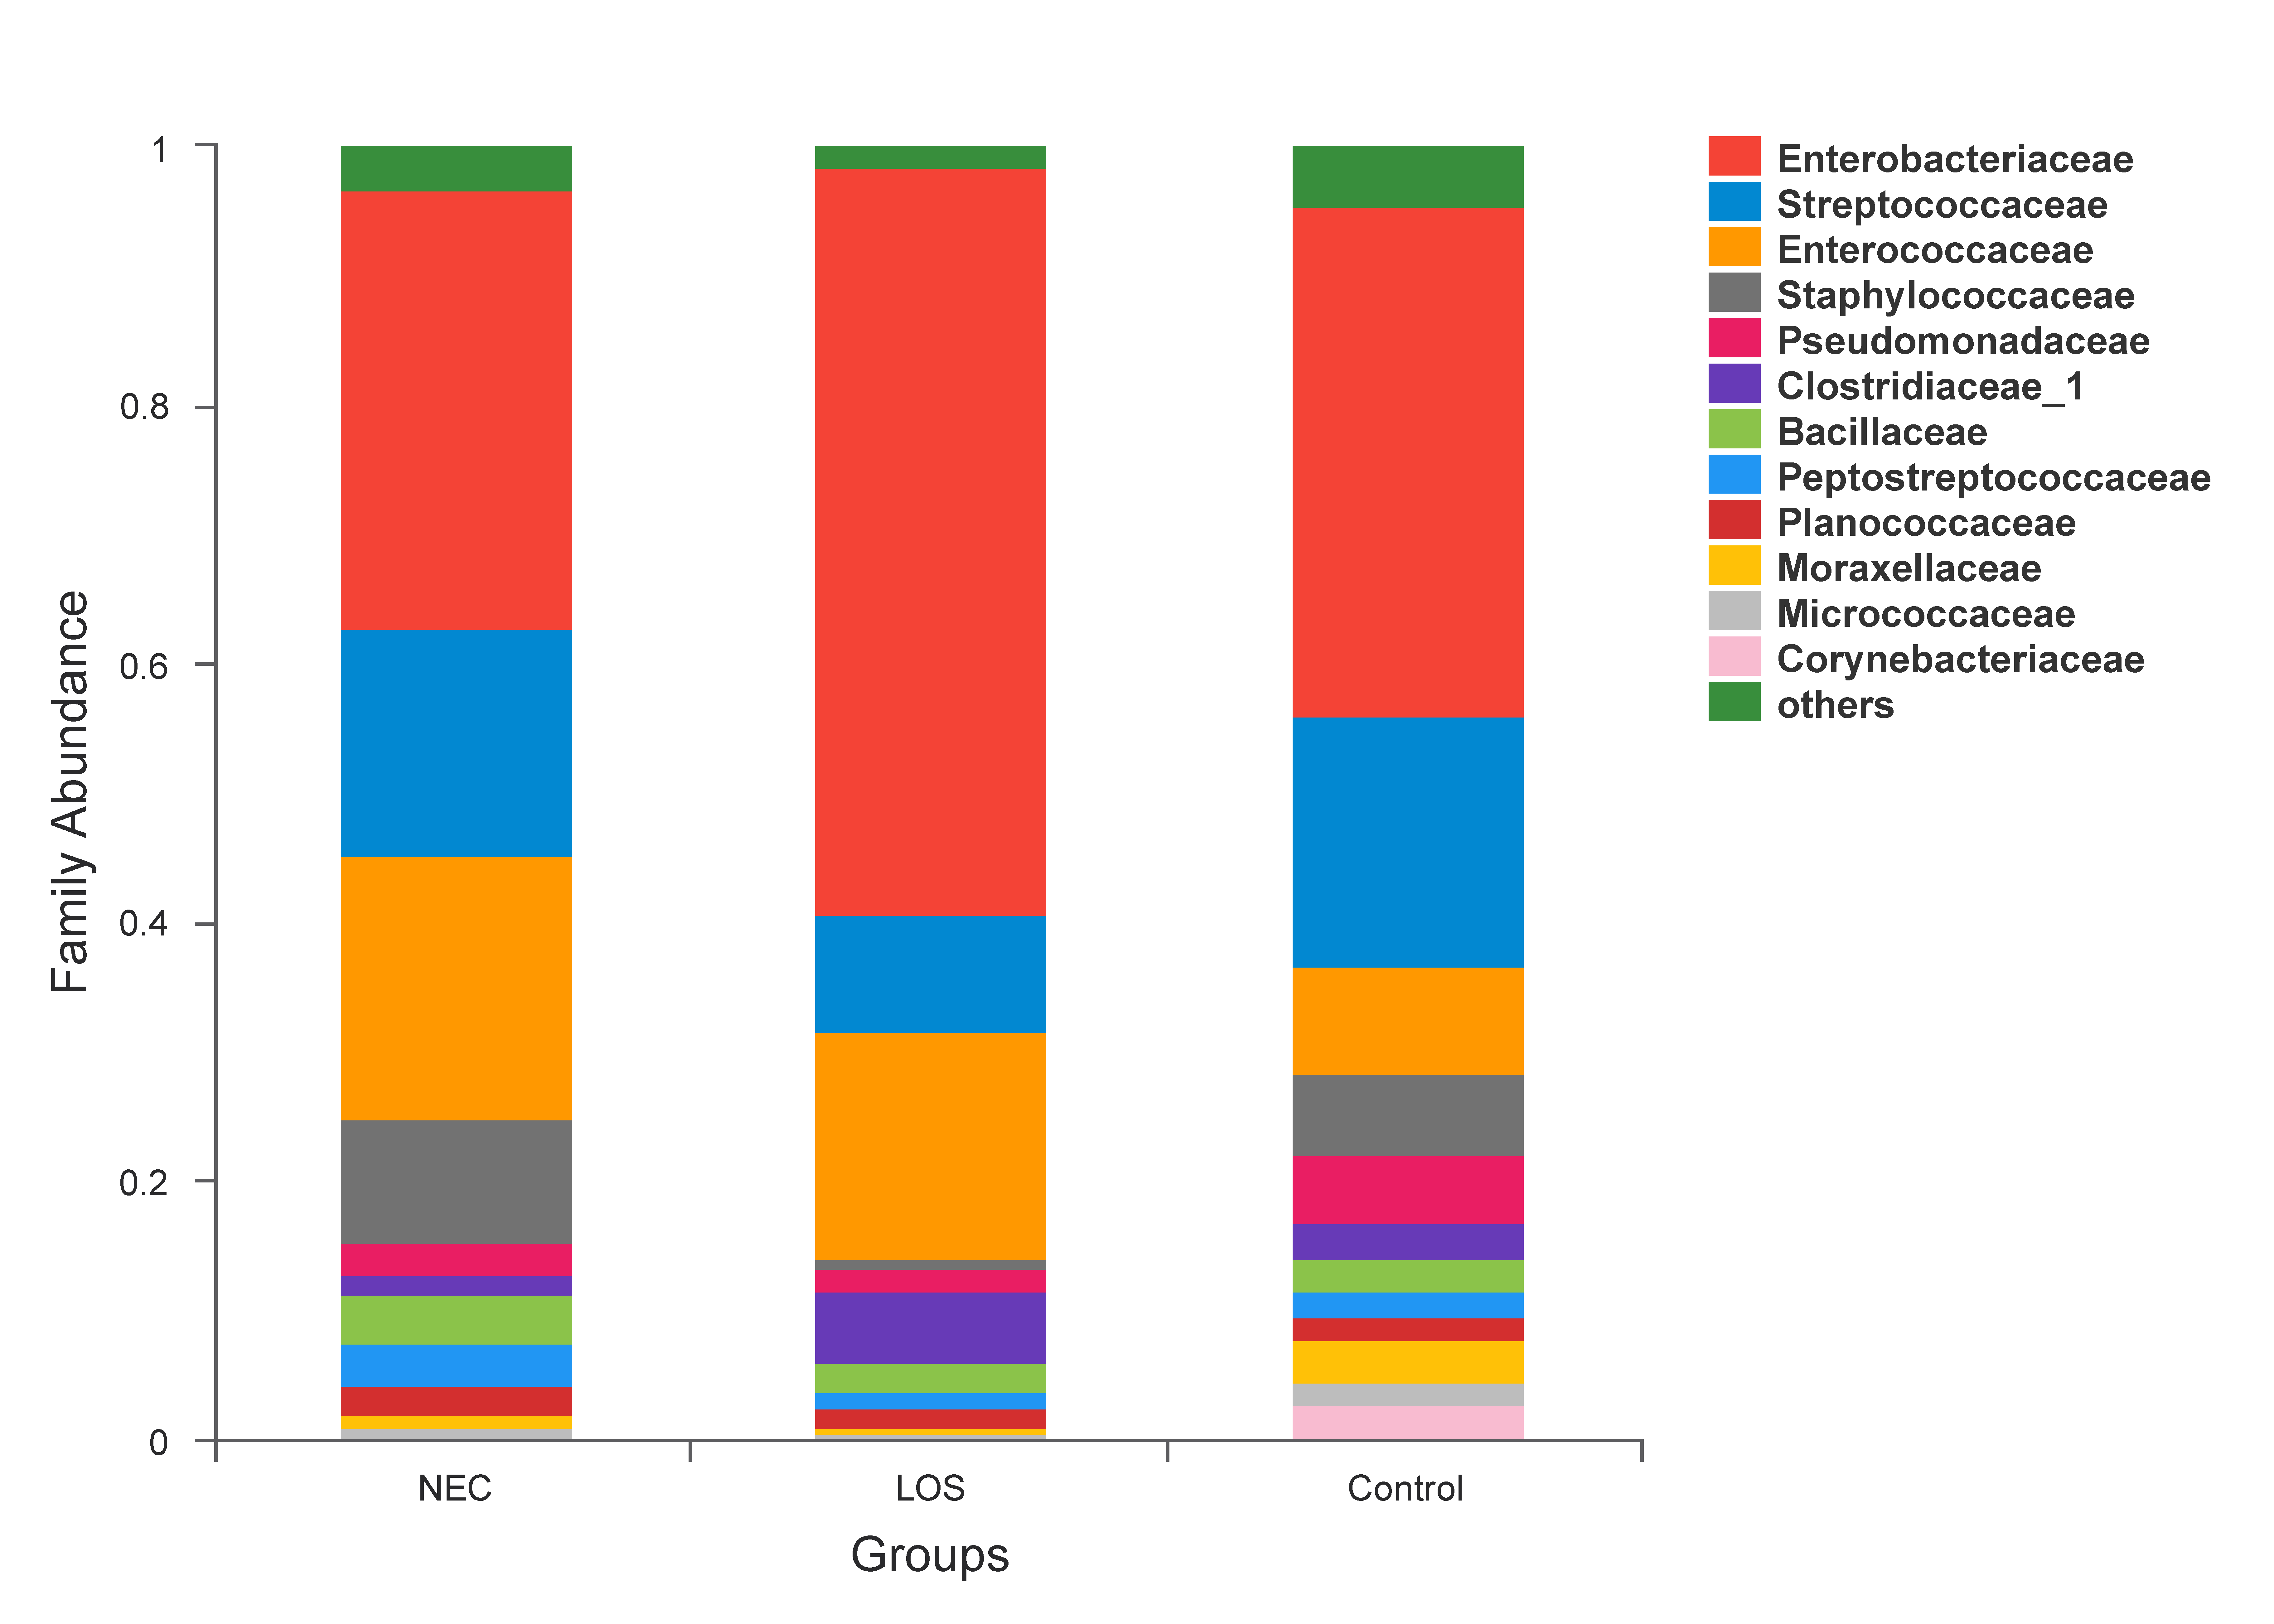
\includegraphics[width=15cm]{2family.pdf}
        \bicaption[科水平上NEC, LOS和对照组患儿菌群相对丰度]
          {纲水平上NEC, LOS和对照组患儿菌群相对丰度。}
          {Relative Abundance of Family in Intestinal Microbiota.}
        \label{fig:2family}
      \end{figure}

    \subsubsection{属(genus)水平}
    属水平上,肠道菌群以克雷伯菌属(\textit{Klebsiella})、肠球菌属(\textit{Enterococcus})、埃希菌-志贺菌属(\textit{Escherichia-Shigella})、乳球菌属(\textit{Lactococcus})、链球菌属(\textit{Streptococcus})、葡球菌属(\textit{Staphylococcus})和假单胞菌属(\textit{Pseudomonas})占主导。克雷伯菌在LOS组丰度最高(\%42.15),且三组丰度差异不显著(p = 0.025);肠球菌属在三组的丰度分别为NEC组20.86\%,LOS组18.14\%,对照组8.45\%,三组间差异不显著(p = 0.105);埃希菌-志贺菌属在三组的丰度分别为NEC组4.83\%,LOS组12.99\%,对照组10.14\%,三组丰度差异不显著(p = 0.291);LOS组乳球菌属丰度3.65\%,显著低于对照组(3.65\%,p = 0.006);链球菌属在三组的丰度分别为NEC组8.67\%,LOS组5.04\%,对照组5.28\%,三组间差异显著(p = 0.0.022);LOS葡球菌属丰度0.15\%,对照组丰度为5.79\%,三组间差异在统计学上非显著(p = 0.526);假单胞菌菌属在三组的丰度分别为NEC组2.41\%,LOS组2.05\%,对照组5.40\%,且三组间丰度存在显著性差异(p = 0.0.039)(图\ref{fig:2genus})。
      %属水平配图
      \begin{figure}[!htp]
        \centering
        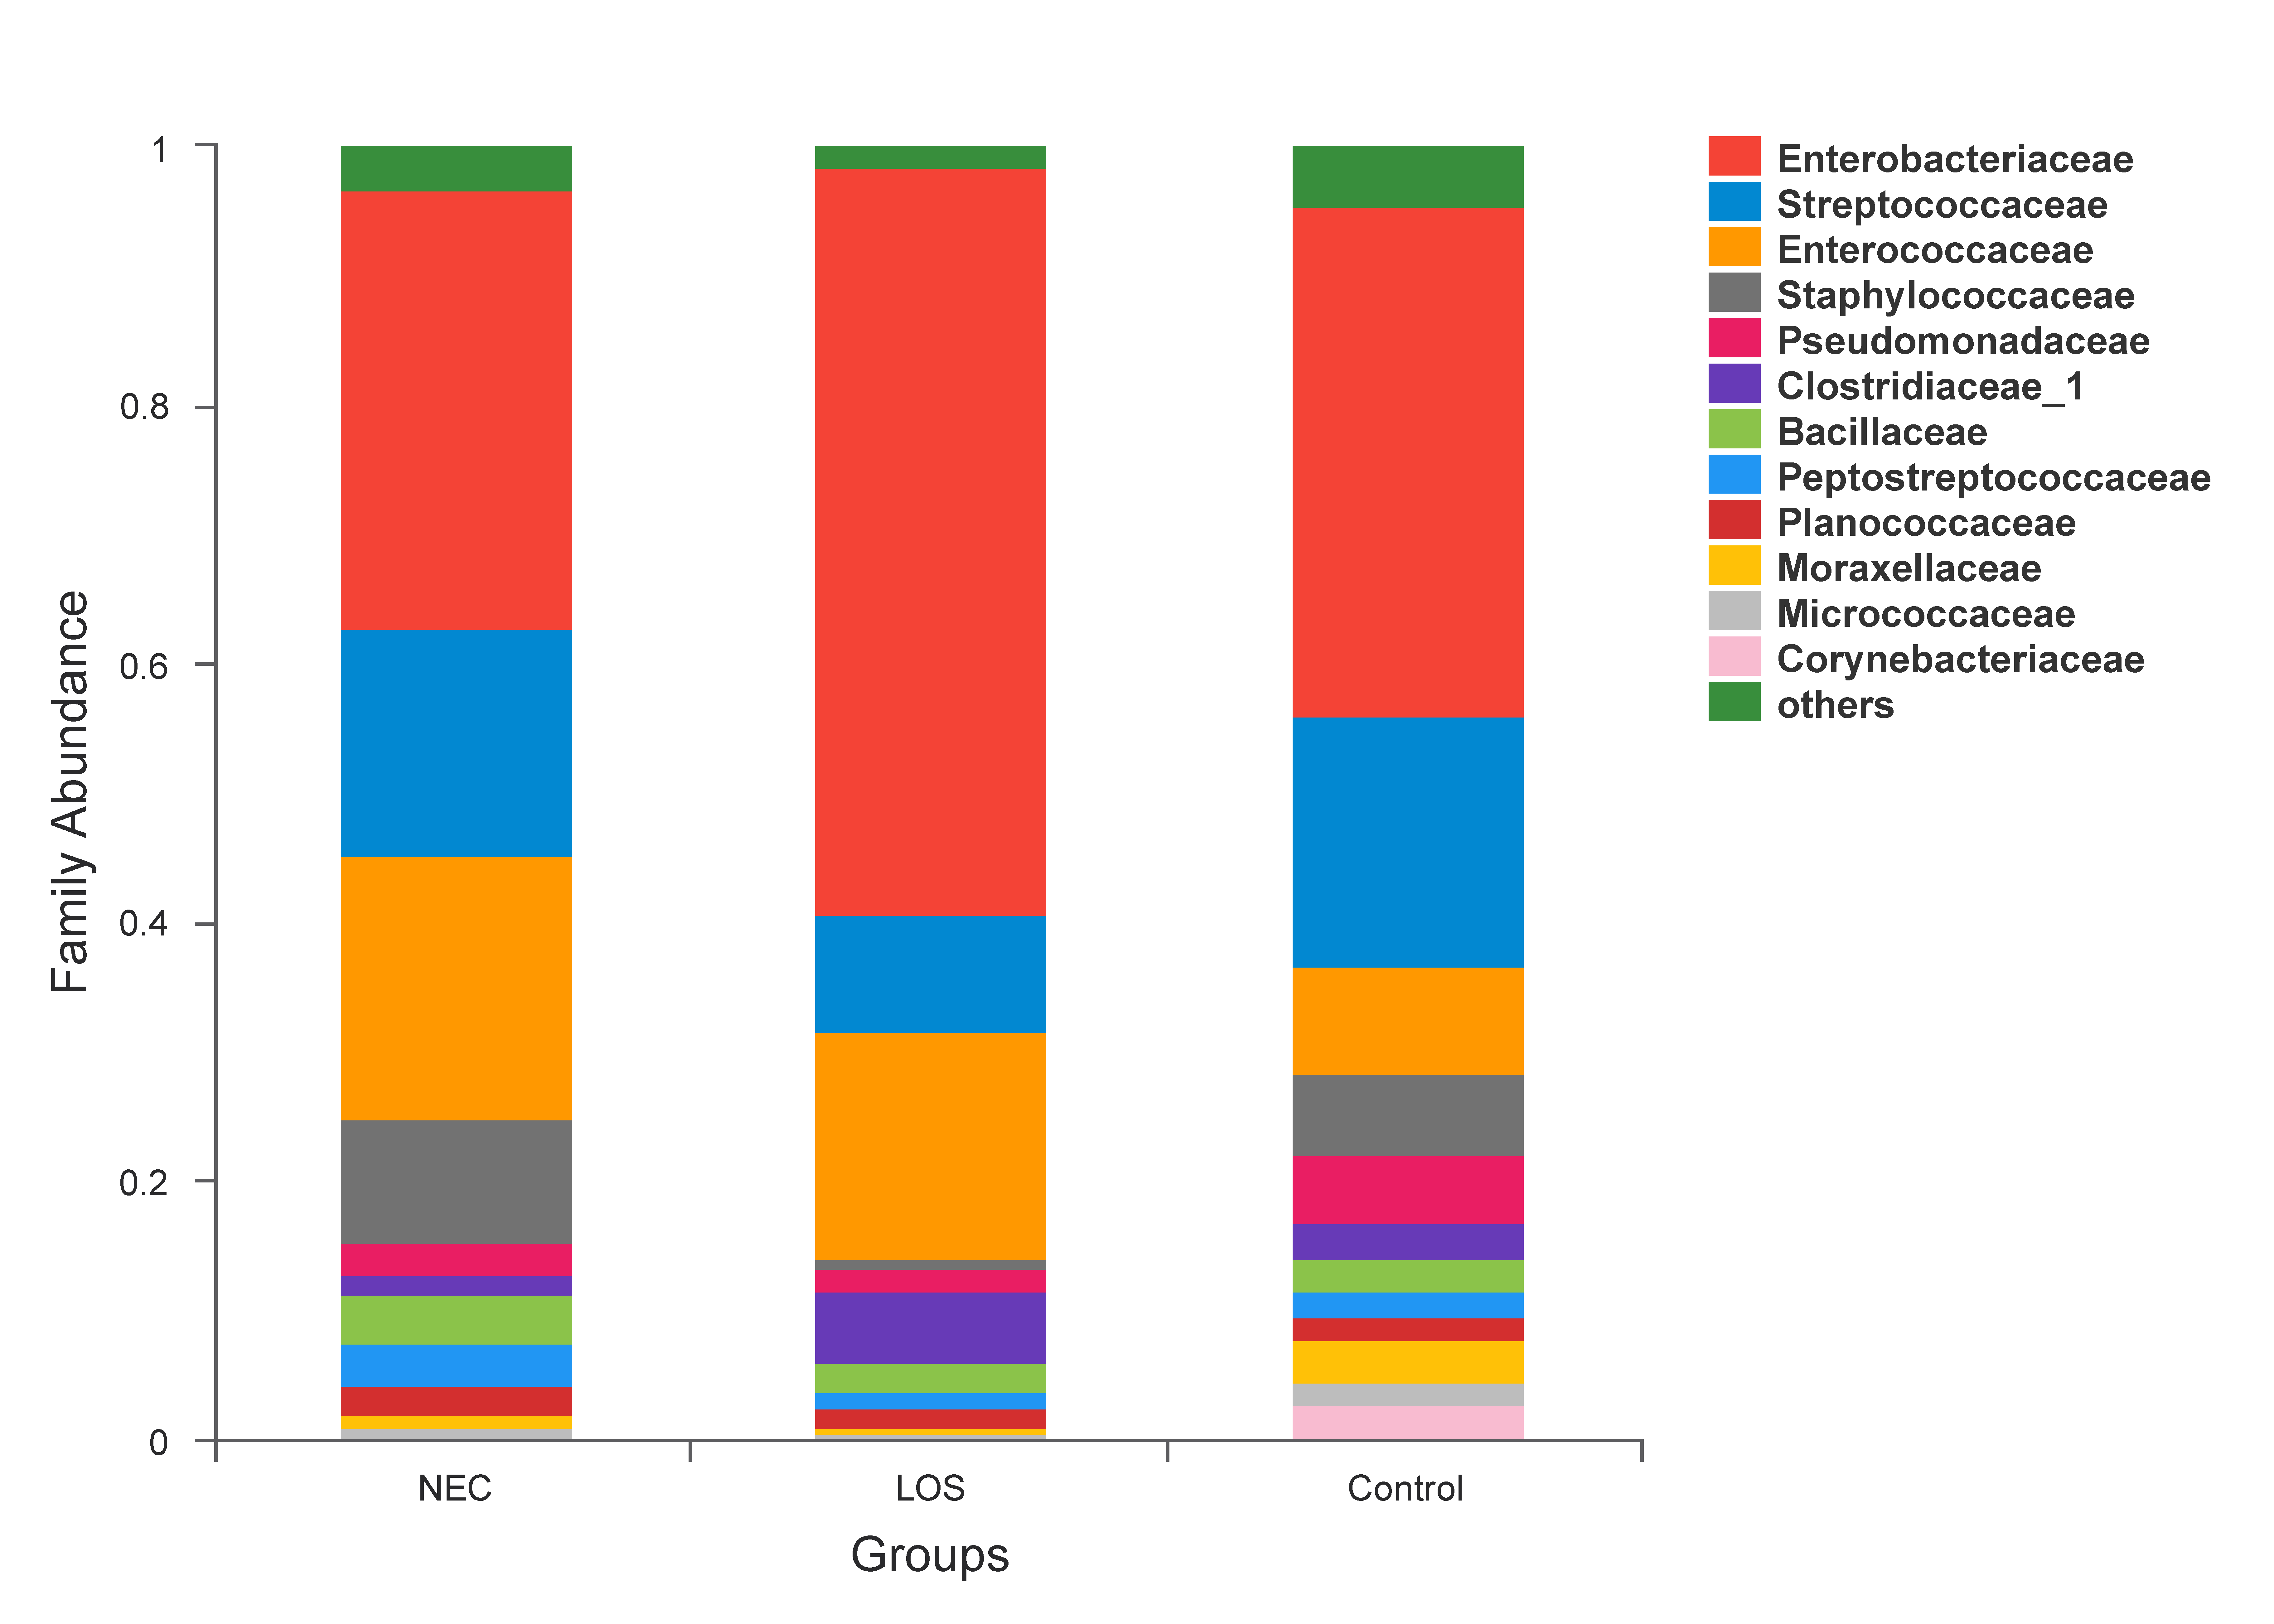
\includegraphics[width=15cm]{2family.pdf}
        \bicaption[属水平上NEC, LOS和对照组患儿菌群相对丰度]
          {属水平上NEC, LOS和对照组患儿菌群相对丰度。}
          {Relative Abundance of Genus in Intestinal Microbiota.}
        \label{fig:2genus}
      \end{figure}

      \subsubsection{多级物种差异判别分析(LEfSe分析)}
      通过LEfSe分析可发现,在NEC组厚壁菌门(\textit{Firmicutes})、芽孢杆菌纲(\textit{Bacillus})、芽孢杆菌XII菌科(\textit{XII\_o\_Bacillales})、微小杆菌属(\textit{Exiguobacterium})和链球菌属(\textit{Streptococcus})的丰度显著增加,同时柔壁菌门(\textit{Tenericutes})、柔壁菌纲(\textit{Mollicutes})、支原体目(\textit{Mycoplasmatales})、支原体科(\textit{Mycoplasmataceae})、尿素原体属(\textit{Ureaplasma})为其独有;而在LOS组,其主导作用的物种为变形菌门(\textit{Proteobacteria})、$\gamma$-变形菌纲(\textit{$\gamma$-Proteobacteria})、肠杆菌目(\textit{Enterobacteriales})、肠杆菌科(\textit{Enterobacteriaceae})、克雷伯菌属(\textit{Klebsiella})为主(图\ref{fig:2lefse})。
        %LEfSe配图
        \begin{figure}[!htp]
          \centering
          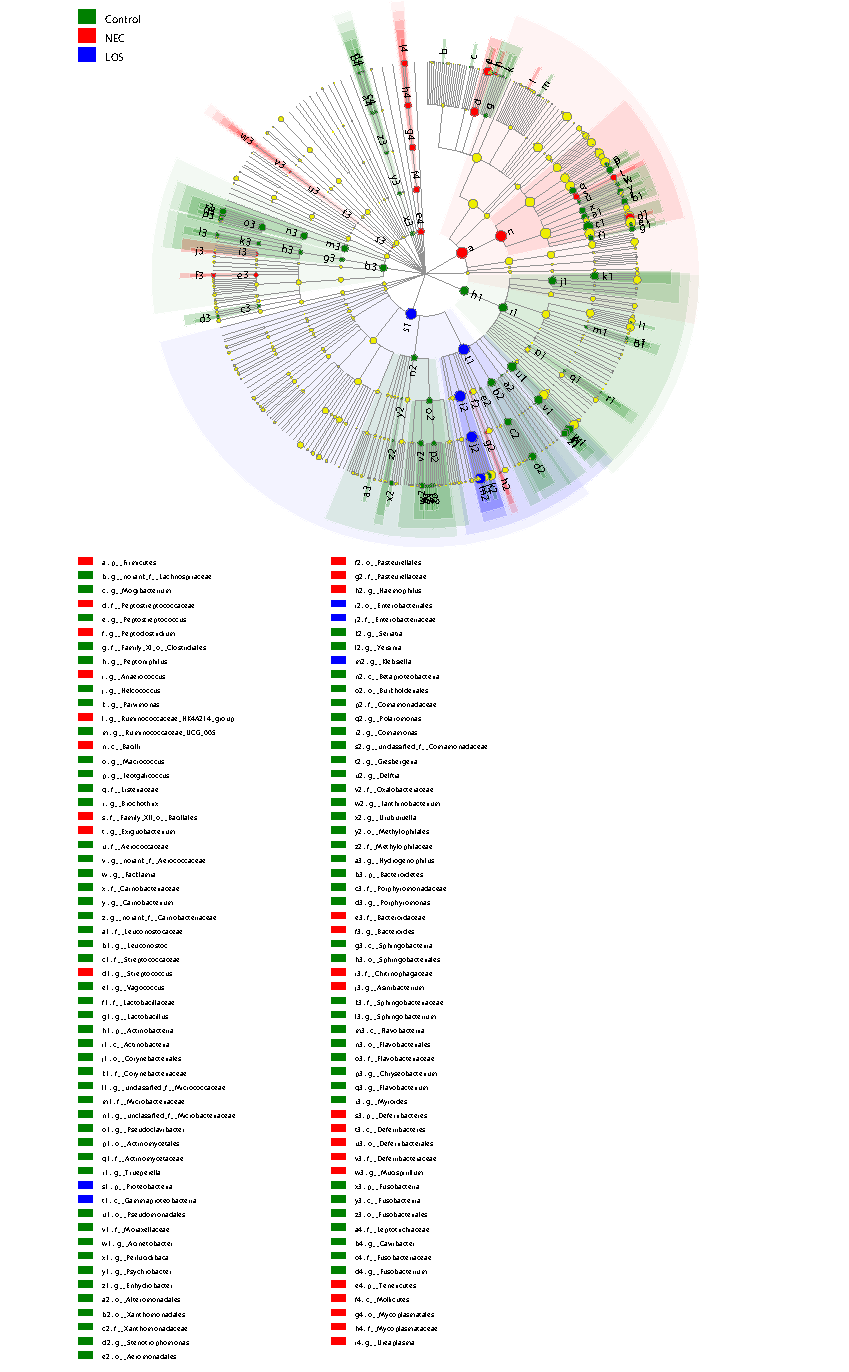
\includegraphics[width=12.5cm]{2lefse.pdf}
          \bicaption[LEfSe分析NEC, LOS和对照组患儿菌群]
            {NEC, LOS和对照组患儿菌群LEfSe进化分支图。绿色代表对照组,红色代表NEC组,蓝色代表LOS组。}
            {Cladogram generated by software LEfSe. Green color represents the control group, red represents the NEC group, and blue represents the LOS group.}
          \label{fig:2lefse}
        \end{figure}

  %多样性
  \subsection{多样性分析和纵向分析}
    \subsubsection{NEC, LOS和对照组患儿间肠道菌群$\alpha$多样性分析}
      基于OTU进行计算,NEC、LOS和对照组Shannon-Wienner指数分别为:1.32,1.16和1.66;三组两两比较,可知LOS组和NEC组、NEC组和对照组shannon指数无统计学差异(分别p = 0.47,p = 0.06),LOS组和对照组之间存在统计学差异(图\ref{fig:2alphadiversity:shannon},p = 0.01)。NEC, LOS 和对照组Simpson指数分别为:0.51,0.53和0.41;三组两两比较,可知LOS组和NEC组Simpson指数无统计学差异(p = 0.77)、NEC组和对照组存在统计学差异(p = 0.03),LOS组和对照组之间存在统计学差异(图\ref{fig:2alphadiversity:simpson},p = 0.02)。
      %alpha多样性图
      \begin{figure}[!htp]
        \centering
          \subcaptionbox{Shannon指数\label{fig:2alphadiversity:shannon}}
            {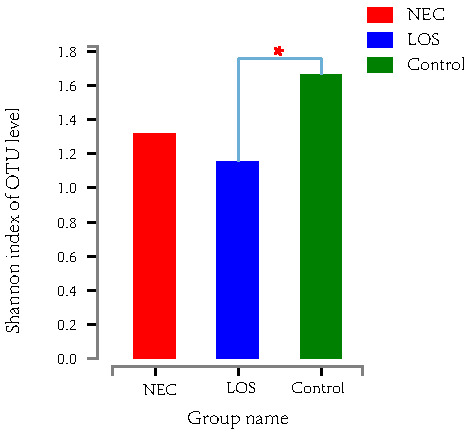
\includegraphics[height=5.5cm]{figure/2shannon.pdf}}
            \hspace{4em}
          \subcaptionbox{Simpson指数\label{fig:2alphadiversity:simpson}}
            {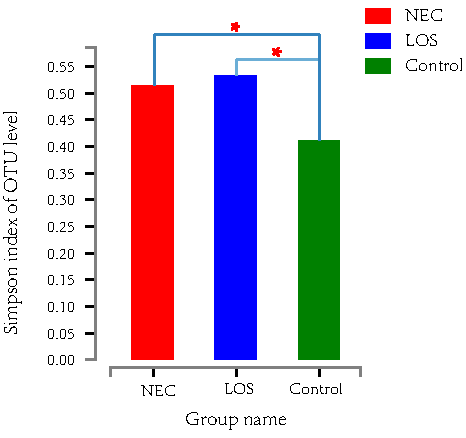
\includegraphics[height=5.5cm]{figure/2simpson.pdf}}
        \bicaption[NEC, LOS和对照组患儿间肠道菌群$\alpha$多样性比较]{通过计算Shannon指数(a)和Simpson(b)指数对NEC, LOS和对照组患儿间肠道菌群$\alpha$多样性分析}{Exploring $\alpha$ diversity by calculation Shannon diversity index(a) and Simpson diversity index(b) among preterm infants with NEC, LOS and Control groups.}
        \label{fig:2alphadiversity}
      \end{figure}
      \subsection{基于$\beta$多样性分析纵向菌群定植模式}
      使用基于weighed unifrac距离的主坐标(PCoA)进行分析发现,NEC、LOS和对照组出生后肠道菌群定植以周为单位进行变化(图\ref{fig:2ingroupweek},(A)PC1 = 69.92\%, PC2 = 15.43\%, ANOSIM r = 0.40, p = 0.001, (B)PC1 = 78.07\%, PC2 = 8.06\%, ANOSIM r = 0.36, p = 0.001, (C)PC1 = 66.59\%, PC2 = 13.18\%, ANOSIM r = 0.40, p = 0.001 ),这与以往研究的结果一致\cite{moles2013bacterial}。
        %分组,按照周来比较pcoa图
          \begin{figure}[!htp]
            \centering
            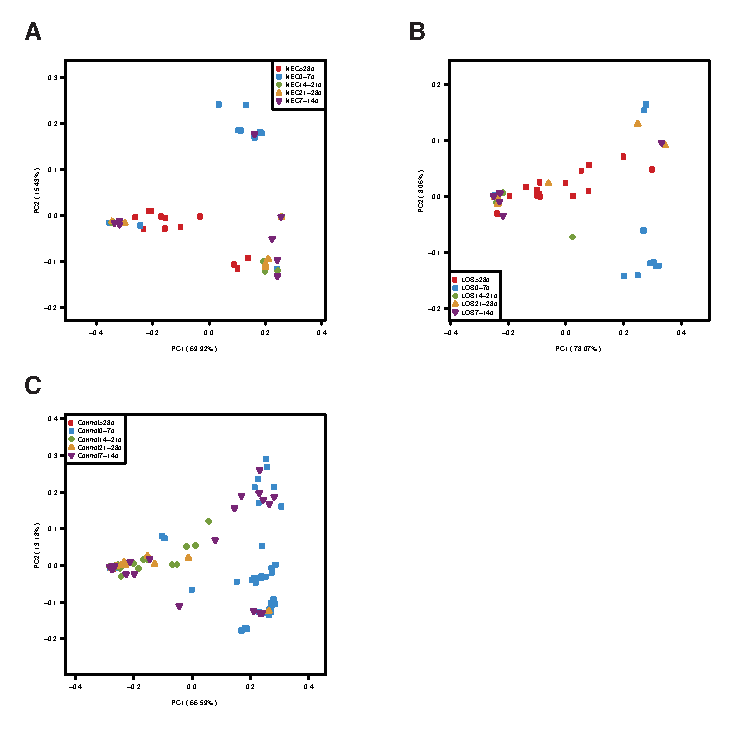
\includegraphics[width=15cm]{2ingroupweek.eps}
            \bicaption[NEC, LOS和对照组组内患儿出生后肠道菌群定植模式变化]
              {使用weighed unifrac距离对出生后肠道菌群定植进行PCoA分析}
              {Post-partum Colonization Pattern by PCoA of Weighed Unifrac Distances}
            \label{fig:2ingroupweek}
          \end{figure}

      三组组间比较以及任意两组比较结果表明,在出生后14天内和21天后,其微生物群定植无明显差异(图\ref{fig:2inweekgroup}(A, B, D, E),ANOSIM (A) r = 0.02, p = 0.797, (B) r = 0.12, p = 0.079, (D) r = 0.21, p = 0.087, (E) r = 0.11, p = 0.183);出生后14到21天即生后第三周,PC1和PC2分别占组间差异的78.18\%和9.29\%(图\ref{fig:2inweekgroup}(C),ANOSIM r = 0.32, p = 0.001),提示菌群模式与NEC发病的可能关联。此外,NEC和对照组的对比显示出生后21到28天即出生后第四周的显著差异(图\ref{fig:2necvscontrol}, ANOSIM r = 0.27, p = 0.030);这表明在NEC病程中存在这菌群的持续失调,尽管在出生后28天后,两组间的差异不显著(ANOSIM r = 0.27, p = 0.052)。
        %分周,按照组来比较pcoa图
          \begin{figure}[!htp]
            \centering
            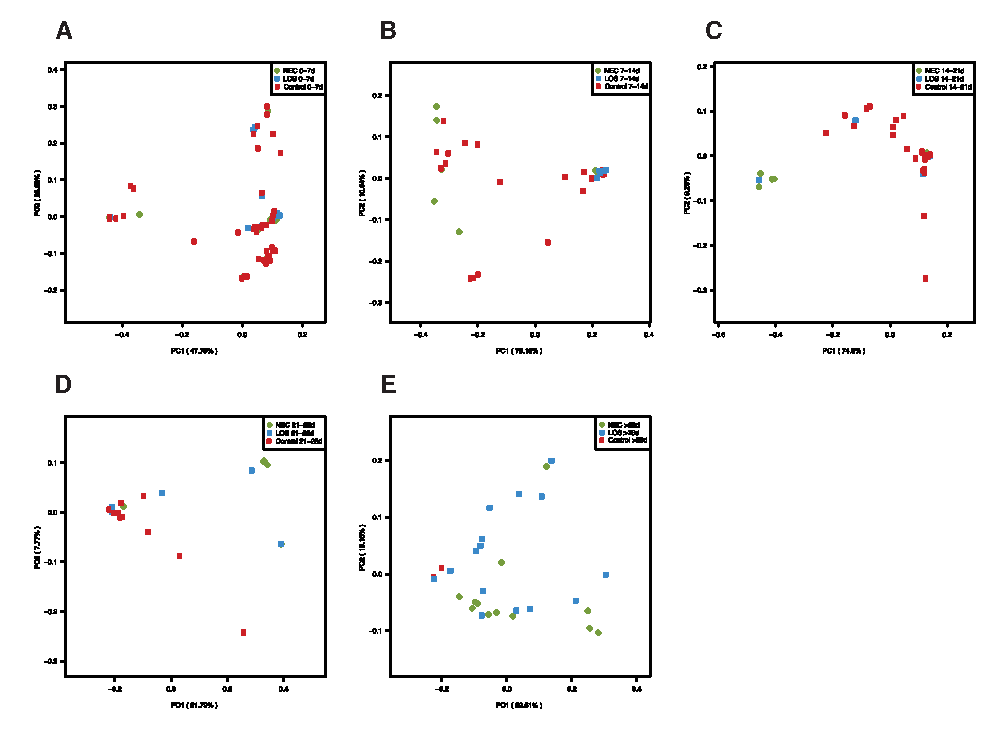
\includegraphics[width=16cm]{2inweekgroup.eps}
            \bicaption[按照日龄对NEC, LOS和对照组患儿间肠道菌群模式分析]
              {使用weighed unifrac距离对三组患儿间肠道菌群模式进行PCoA分析。三组患儿在出生后0到7天菌群分布相似。但在出生后14天开始,菌群模式出现显著差异,而此时也是NEC常见的发病时间。}
              {The PCoA of Microbiota Colonization Analysis on a Weekly Basis after Birth. The colonization patterns within 14 days after birth were similar among NEC, LOS and Control groups. However, after the 14th day after birth, the diversity differed among three groups, which was the time when most NEC occurs. }
            \label{fig:2inweekgroup}
          \end{figure}
        %NEC和对照组单独比较
          \begin{figure}[!htp]
            \centering
            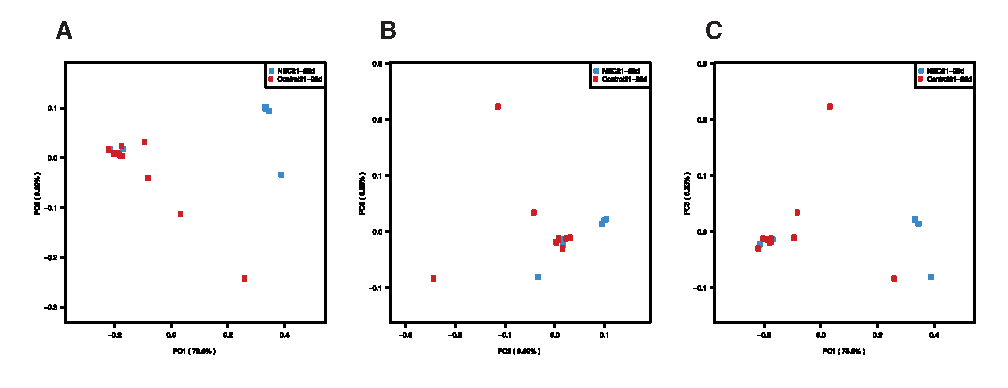
\includegraphics[width=16cm]{2necvscontrol.eps}
            \bicaption[NEC和对照组患儿肠道菌群模式比较]
              {使用weighed unifrac距离对NEC和对照组患儿肠道菌群模式进行PCoA分析。}
              {The PCoA of Microbiota Colonization Analysis between NEC and Control groups.}
            \label{fig:2necvscontrol}
          \end{figure}

      另外,为排除组内个体间差异对于分析结果的潜在影响,本研究对于每个NEC患儿进行单病例的微生物组成PCoA分析,并发现其各自肠道微生物定植随着出生后时间推移的显著模式(图\ref{fig:2neccases},ANOSIM (A) r = 0.26, p = 0.01, (B) r = 1.00, p = 0.035, (C) r = 0.610, p = 0.014, (D) r = 0.09, p = 0.008)。
        %NEC case by cases
          \begin{figure}[!htp]
            \centering
            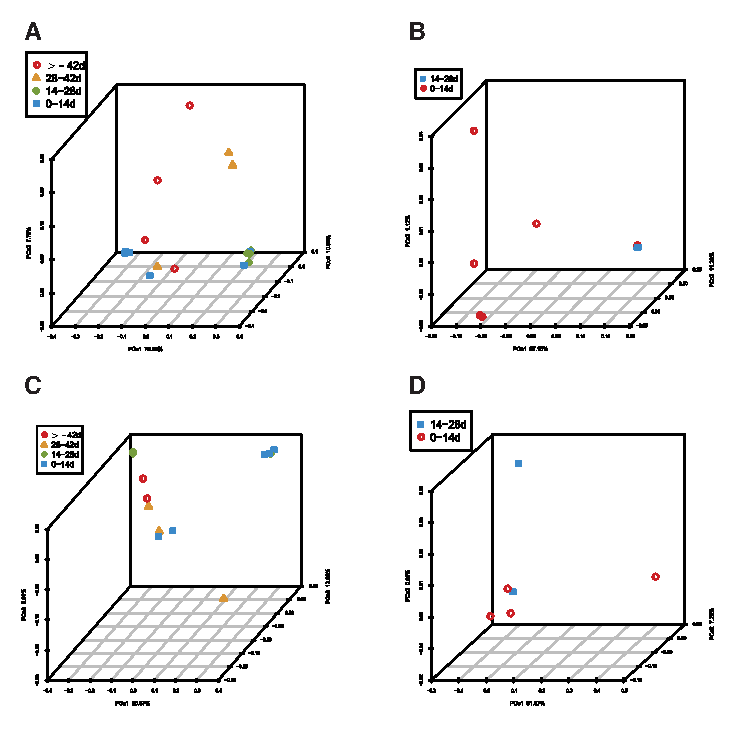
\includegraphics[width=16cm]{2neccases.eps}
            \bicaption[三名NEC患儿出生后菌群定植模式]
              {使用weighed unifrac三名NEC患儿出生后菌群定植模式进行PCoA分析。(A)NEC patient No.1, (B)NEC patient No.1, (C)NEC patient No.1, (D)NEC patient No.1}
              {The PCoA OF post-partum colonization of each NEC patient. (A)NEC patient No.1, (B)NEC patient No.1, (C)NEC patient No.1, (D)NEC patient No.1}
            \label{fig:2neccases}
          \end{figure}

\section{讨论}
在人类肠道黏膜中定植了超过10万亿个微生物\cite{Ley2006},并在方方面面影响人类的健康\cite{Sekirov2009}。肠道微环境紊乱可能扰乱人体稳态并导致各种疾病,包括肥胖\cite{Liu2017}),IBD\cite{Ley2006},心血管疾病\cite{Wang2011},以及精神障碍\cite{Rogers2016}等。虽然早期细菌定植对人类健康的长期影响仍然缺乏证据,但它仍然是新生儿出生后健康或某些疾病易感性的重要因素。到目前为止,少有研究关注NEC菌群的纵向发展,另外,对于新生儿晚期败血症(Late-Onset Sepsis,LOS)的菌群研究也十分有限。近期有研究发现NEC的致病菌与梭菌(\textit{Clostridium})增殖相关\cite{hosny2017updating}。然而,特定病原体尚未确定;2013年的一项研究表明,在生命的4-9天内早期的生态失调可能与NEC病理生理学密切相关\cite{morrow2013early}。因此,为在菌群层面提供对其病因学的新见解,本研究致力于探究肠道菌群定植的发展模式,而非寻找单一病原体。

本研究描述并比较了NEC和LOS早产儿及其匹配对照组出生后肠道菌群的定植模式的发展。我们对192个肠道标本中的16S rRNA基因进行了测序:包括NEC早产儿的46个标本,LOS早产儿的42个标本,以及对照组的103个标本。使用Illumina-MiSeq平台为所有样品生成了总共7,472,400个序列,并检测出一些在自然环境下较为稀有的OTU。

本研究显示早产儿在NEC发病期间存在丰富的变形菌;另外,数据显示,NEC患者中的厚壁菌门丰富(59.79\%),而对照组和LOS组则为变形菌。此外,NEC患者在发病前分别在1-3天和3-7天内肠球菌和葡萄球菌的平均丰度最高,相比对照组对照组相比增加了克雷伯氏菌和葡萄球菌的丰度也更高。这些发现表明潜在的致​​病性葡萄球菌属在NEC的发病机理中可能的作用以及常规致病物种如金黄色葡萄球菌(\textit{Staphylococcus areus})和溶血性葡萄球菌(\textit{Staphylococcus haemolyticus})。革兰氏阴性克雷伯氏菌丰度增加的趋势表明LPS的作用,作为TRL-4的配体其能促进体外Caco-2胞吞转运作用\cite{panigrahi1996escherichia},并增加细菌易位\cite{Deitch1987}。

此外,LOS组中显着的肠球菌表明高级别抗生素治疗会对菌群平衡产生较大影响。尽管脓毒症中确切的微生物群组成仍有待通过动物研究来阐明\cite{Hand2012a,Sekirov2009},脓毒症,免疫反应和微生物群破坏的机制及其后果可能有助于我们对败血症进展的理解并帮助制定战略性预防性解决方案。在一项关于成人的临床研究中,系统性炎症反应综合症对患者肠道厌氧菌减少和肠道致病菌增加与更高的败血症并发症和更高对死亡率相关\cite{Shimizu2011};菌群的早期异常定植也与医院相关事件相关\cite{Dutta2014},包括机械通气和抗生素治疗\cite{Moles2013}。虽然我们相对较小的样本量仅显示特定菌属与败血症发病相关的证据有限,但脓毒症患儿的宿主 - 微生物群 - 病原体相互作用值得进一步研究。

另一项研究发现,早产儿肠道微生物群的定植和突然变化可能是分娩方式,喂养类型和孕龄的结果\cite{Dutta2014}。以往研究在早产儿中观察到从芽孢杆菌,$\gamma$芽孢杆菌到梭菌的一系列细菌\cite{LaRosa2014})的先后主导作用在本研究内在包括LOS患者在内的大多数研究受试者中也观察到。本研究证实了出生后以周为时间单位的细菌定植模式,并发现每组肠道微生物群在不同组患儿间存在的显着差异。此外,本研究数据显示,在出生后第14天,NEC和对照组之间的肠道微生物群显着不同,尽管在出生后的前14天内具有相似的定植模式(图\ref{fig:2ingroupweek}),Anosim r = 0.32 p = 0.001),表明肠道微生态失调与NEC发病之间的强相关性。最后,肠道微生物群在出生后第21天至第28天的差异(图\ref{fig:2ingroupweek},ANOSIM r = 0.27,p = 0.030)表明在NEC进展期间持续的生态失调,这与之前的横断面研究一致\cite{Wang2009}。

\section{结论}
多年来,临床医生和科研工作者在不断努力探究NEC和LOS与肠道菌群的相关性。虽然尚未阐明特定的病原体或微生物模式,但现有的研究结果有助于改善临床策略,并最大限度地减少早产儿的并发症。

本研究使用高通量测序描述、比较和分析早产儿出生后肠道微生物群的动态模式在NEC和LOS早产儿中的作用的研究。我们的研究结果结果支持了“肠道生态失调假说”,即肠道微生物群的“异常动态定制模式”是早产儿NEC和LOS发生进展的重要因素。

肠道菌群失调和潜在致病菌的过度增殖与NEC和LOS进展至关重要,抗生素(特别是氨基糖苷类抗生素),可以减少早产儿肠道微生物群落的丰度和多样性。

本研究发现早产儿出生后以周为时间单位的肠道菌群变化模式。早产儿出生后第2周起,肠道菌群定植模式出现紊乱并逐渐发展为早产特定感染,NEC和LOS分别呈现不同的纵向变化规律,包括不同致病菌属的丰度增加及菌群多样性不同程度的降低,并且与临床变化相关。

本研究以及其他类似相关研究在肠道菌群动态变化和构成方面提供了早产儿NEC和LOS发生和发展的证据,从而帮助其早期预防、诊断和治疗,以降低其发病率和严重程度。

当然,本研究有其局限性。首先,本研究中的所有婴儿均采用配方奶进行喂养,因此无法评估人类母乳的保护作用。由于所有患儿入院时均的经验性抗生素方案,因此经验型抗生素对对肠道微生物群的影响无法完全避免。但是,三组横向及纵向比较研究方法可以最大程度找到差异影响因素。此外,NEC和LOS组样本量比较小。本研究结果仍需要在更大样本量的验证。

%# -*- coding: utf-8-unix -*-
% !TEX program = xelatex
% !TEX root = ../thesis.tex
% !TEX encoding = UTF-8 Unicode
\chapter{常见问题}
\label{chap:faq}

{\bfseries{}Q:我是否能够自由使用这份模板?}

A:这份模板以Apache License 2.0开源许可证发布,请遵循许可证规范。

{\bfseries{}Q:我的论文是Word排版的,学校图书馆是不是只收 \LaTeX 排版的论文?}

A:当然不是,Word版论文肯定收。

{\bfseries{}Q:我的论文是 \LaTeX 排版的,学校图书馆是不是只收Word排版的论文?}

A:当然不是,PDF版的电子论文是可以上交的。是否要交Word版就看你导师的喜好了。

{\bfseries{}Q:为什么屏幕上显示的左右页边距不一样?}

A:模板默认是双面打印,迎面页和背面页的页边距是要交换的,多出来的那一部分是留作装订的。

{\bfseries{}Q:为什么在参考文献中会有“//”符号?}

A:那就是国标GBT7714参考文献风格规定的。但可以使用 gbpunctin=false 选项将其还原成 in:,进一步可以在导言区加入\verb+\DefineBibliographyStrings{english}{in={}}+将其去掉。

{\bfseries{}Q:为什么参考文献中会有[s.n.],[S.l], [EB/OL]等符号?}

A: 那也是国标GBT7714参考文献风格定义的。[s.n.]表示出版者不祥,[S.l]表示出版地不祥,[EB/OL]表示引用的参考文献类型为在线电子文档。但可以使用gbpub=false 选项将其缺省补充的出版项[s.n.]等去掉。也可以使用选项 gbtype=false 将参考文献类型标识去掉。

{\bfseries{}Q:如何获得帮助和反馈意见?}

A:你可以通过\href{https://github.com/sjtug/SJTUThesis/issues}{在github上开issue}
、在\href{https://bbs.sjtu.edu.cn/bbsdoc?board=TeX_LaTeX}{水源LaTeX版}发帖反映你使用过程中遇到的问题。

{\bfseries{}Q:使用文本编辑器查看tex文件时遇到乱码?}

A:请确保你的文本编辑器使用UTF-8编码打开了tex源文件。

{\bfseries{}Q:在CTeX编译模板遇到“rsfs10.tfm already exists”的错误提示?}

A:请删除\verb+X:\CTEX\UserData\fonts\tfm\public\rsfs+下的文件再重新编译。问题讨论见\href{https://bbs.sjtu.edu.cn/bbstcon,board,TeX_LaTeX,reid,1352982719.html}{水源2023号帖}。

{\bfseries{}Q:升级了TeXLive 2012,编译后的文档出现“minus”等字样?}

A:这是xltxtra和fontspec宏包导致的问题。学位论文模板从0.5起使用metatlog宏包代替xltxtra生成 \XeTeX 标志,解决了这个问题。

{\bfseries{}Q:为什么在bib中加入的参考文献,没有在参考文献列表中出现?}

A: bib中的参考文献条目,常通过\verb+\cite+或\verb+\parencite+或\verb+\supercite+或\verb+\textcite+等命令在正文中引用进而加入到参考文献列表中。当需要将参考文献条目加入到文献表中但又不引用可以使用\verb+\nocite+命令,当nocite参数为*时则引入bib中的所有文献。
%\verb+\upcite+ 是哪个宏包的?之前没有见过

{\bfseries{}Q:我可以使用Sublime Text编写学位论文吗?}

A: 可以。首先\href{https://www.sublimetext.com/}{下载}并安装Sublime Text,然后安装
\href{https://packagecontrol.io/installation}{Package Control},
之后按\verb|ctrl+shift+p|或者\verb|cmd+shift+p|调出命令窗口,
输入\verb|install|,选择\textit{Package Control: Install Package},按回车,
稍等片刻,等待索引载入后会弹出选项框,输入\verb|LaTeXTools|并回车,即可成功安装插件。
之后只需要打开\verb|.tex|文件,按\verb|ctrl+b|或者\verb|cmd+b|即可编译,
如有错误,双击错误信息可以跳转到出错的行。

{\bfseries{}Q:在macTex中,为什么pdf图片无法插入?}

A:如果报错是“pdf: image inclusion failed for "./figure/chap2/sjtulogo.pdf".”,则采取以下步骤

\begin{lstlisting}[basicstyle=\small\ttfamily, caption={编译模板}, numbers=none]
brew install xpdf
wget http://mirrors.ctan.org/support/epstopdf.zip
unzip epstopdf.zip
cp epstopdf/epstopdf.pl /usr/local/bin/
cd figure/chap2
pdftops sjtulogo.pdf
epstopdf sjtulogo.ps
pdfcrop sjtulogo.pdf
mv sjtulogo.pdf backup.pdf
mv sjtulogo-crop.pdf sjtulogo.pdf
\end{lstlisting}

{\bfseries{}Q:为什么维普等查重系统无法识别此模板生成的 pdf 内所有的中文?}

A: 中文无法识别的情况多半是由于使用了 ShareLaTeX 的原因,请尝试使用 TexStudio 等软件在本地进行编译。
如果使用 TeXstudio 请在 Preferences-Build 中将 Default Compiler 和 Default Bibliography Tool 分别改为 XeLaTeX 和 Biber。

{\bfseries{}Q:如何向你致谢?}

A: 烦请在模板的\href{https://github.com/sjtug/SJTUThesis}{github主页}点击“Star”,我想粗略统计一下使用学位论文模板的人数,谢谢大家。非常欢迎大家向项目贡献代码。

\addtocontents{toc}{\protect\setcounter{tocdepth}{0}} %此行要放在最后一章前面,为了把附录的section省略!
%# -*- coding: utf-8-unix -*-
% !TEX program = xelatex
% !TEX root = ../thesis.tex
% !TEX encoding = UTF-8 Unicode
%%==================================================
%% conclusion.tex for SJTUThesis
%% Encoding: UTF-8
%%==================================================

\begin{summary}

这里是全文总结内容。

2015年2月28日,中央在北京召开全国精神文明建设工作表彰暨学雷锋志愿服务大会,公布全国文明城市(区)、文明村镇、文明单位名单。上海交通大学荣获全国文明单位称号。         

全国文明单位这一荣誉是对交大人始终高度重视文明文化工作的肯定,是对交大长期以来文明创建工作成绩的褒奖。在学校党委、文明委的领导下,交大坚持将文明创建工作纳入学校建设世界一流大学的工作中,全体师生医护员工群策群力、积极开拓,落实国家和上海市有关文明创建的各项要求,以改革创新、科学发展为主线,以质量提升为目标,聚焦文明创建工作出现的重点和难点,优化文明创建工作机制,传播学校良好形象,提升社会美誉度,显著增强学校软实力。2007至2012年间,上海交大连续三届荣获“上海市文明单位”称号,成为创建全国文明单位的新起点。         

上海交大自启动争创全国文明单位工作以来,凝魂聚气、改革创新,积极培育和践行社会主义核心价值观。坚持统筹兼顾、多措并举,将争创全国文明单位与学校各项中心工作紧密结合,着力构建学校文明创建新格局,不断提升师生医护员工文明素养,以“冲击世界一流大学汇聚强大精神动力”为指导思想,以“聚焦改革、多元推进、以评促建、丰富内涵、彰显特色”为工作原则,并由全体校领导群策领衔“党的建设深化、思想教育深入、办学成绩显著、大学文化丰富、校园环境优化、社会责任担当”六大板块共28项重点突破工作,全面展现近年来交大文明创建工作的全貌和成就。         

进入新阶段,学校将继续开拓文明创建工作新格局,不断深化工作理念和工作实践,创新工作载体、丰富活动内涵、凸显创建成效,积极服务于学校各项中心工作和改革发展的大局面,在上级党委、文明委的关心下,在学校党委的直接领导下,与时俱进、开拓创新,为深化内涵建设、加快建成世界一流大学、推动国家进步和社会发展而努力奋斗!       

上海交通大学医学院附属仁济医院也获得全国文明单位称号。      

\end{summary}


\appendix % 使用英文字母对附录编号

% 附录内容,本科学位论文可以用翻译的文献替代。
%%# -*- coding: utf-8-unix -*-
% !TEX program = xelatex
% !TEX root = ../thesis.tex
% !TEX encoding = UTF-8 Unicode
\chapter{原始数据与源代码存档}

\section{原始测序数据存档}
坏死性小肠结肠炎(NEC)肠道菌群MiSeq测序原始数据:


\subsection{Mac OS X}

Mac用户可以从MacTeX主页\footnote{\url{https://tug.org/mactex/}}下载MacTeX。
也可以通过brew包管理器\footnote{\url{http://caskroom.io}}安装MacTeX。

\begin{lstlisting}[basicstyle=\small\ttfamily, numbers=none]
brew cask install mactex
\end{lstlisting}

\subsection{Linux}

建议Linux用户使用TeXLive主页\footnote{\url{https://www.tug.org/texlive/}}的脚本来安装TeXLive。
以下命令将把TeXLive发行版安装到当前用户的家目录下。
若计划安装一个供系统上所有用户使用的TeXLive,请使用root账户操作。

\begin{lstlisting}[basicstyle=\small\ttfamily, numbers=none]
wget http://mirror.ctan.org/systems/texlive/tlnet/install-tl-unx.tar.gz
tar xzvpf install-tl-unx.tar.gz
cd install-tl-20150411/
./install-tl
\end{lstlisting}

\section{安装中文字体}

\subsection{Mac OS X、Deepin}

Mac和Deepin用户双击字体文件即可安装字体。

\subsection{RedHat/CentOS用户}

RedHat/CentOS用户请先将字体文件复制到字体目录下,调用fc-cache刷新缓存后即可在TeXLive中使用新字体。

\begin{lstlisting}[basicstyle=\small\ttfamily, numbers=none]
mkdir ~/.fonts
cp *.ttf ~/.fonts				# 当前用户可用新字体
cp *.ttf /usr/share/fonts/local/	# 所有用户可以使用新字体
fc-cache -f
\end{lstlisting}

%%# -*- coding: utf-8-unix -*-
% !TEX program = xelatex
% !TEX root = ../thesis.tex
% !TEX encoding = UTF-8 Unicode
\chapter{原始数据与源代码存档}

\section{原始测序数据存档}
\textbf{坏死性小肠结肠炎(NEC)肠道菌群MiSeq测序原始数据}
\textbf{儿科炎症性肠病肠道菌群MiSeq测序原始数据}

\section{论文相关源代码和原始图标存档}
\textbf{源代码\footnote{本论文使用 \LaTeX 编译生成}}
尝试引用\cite{collier2005innate}

\textbf{原始图片和表格}

%# -*- coding: utf-8-unix -*-
% !TEX program = xelatex
% !TEX root = ../thesis.tex
% !TEX encoding = UTF-8 Unicode
\chapter{综述\quad 肠道菌群研究中粪便样品取样与保存方法}
\label{app:review}

\begin{center} \textbf{Sampling and Storage Methods of Fecal samples \\ in human intestinal microbiome study}
\end{center}

\begin{description}
    \item[摘要] 随着高通量测序技术(next generation sequencing, NGS )的飞速发展,肠道菌群得以被更深入的研究。肠道内容物和粪便样品有着取样便捷、代表性强等特点,因此常被作为肠道菌群研究中的主要研究对象;而样品的收集和保存方法很大程度上影响其内部菌群结构和多样性,从而决定了后续测序分析的准确性。该文将就现今常用的肠道菌群研究中粪便样品的取样和保存方法进行综述。
    \item[关键词] 肠道菌群;高通量测序;肠道内容物;粪便;取样
    \item[基金项目] 国家自然科学基金(项目编号81771630)
    \item[Abstract]With the rapid development of high-throughput sequencing (NGS) technique, intestinal microbiome could be studied more deeply. Intestinal contents and fecal samples have the characteristics of convenient sampling and strong representation, so they are often used as the main research objects in the study of intestinal microbiota. The method of collecting and storage of samples are very important to affect the internal flora structure and diversity, which determines the accuracy of subsequent sequencing analysis. This review summarizes the sampling and storage methods of fecal samples in the study of intestinal microbiome.
    \item[Key Words]Intestinal Microbiome;High Throughput DNA Sequencing;Intestinal Contents;Feces;Specimen Collection
    \item[Fundings]National Natural Science Foundation of China (Project No. 81771630)
\end{description}


肠道菌群是广泛存在于人类和其他动物(包括昆虫)的肠道中的微生物所组成的复杂群落;在正常人体肠道中,存在至少1000种菌种。肠道菌群宏基因组是肠道菌群的所有基因组的总和,它包含了超过三百万个基因\cite{Saxena2016}。肠道与人体内其他部位相比,细菌数量最多、物种丰度最高\cite{Willey2013}。

越来越多的研究表明,人体肠道菌群的早期定植、构成、转换模式、代谢特点和免疫应答模式与肥胖、糖尿病、炎症性肠病、自闭症等多种疾病的发生与发展相关\cite{Li2016c,lozupone2012diversity}。因此,肠道菌群研究对于疾病发病机制及临床防治的重要性不言而喻。粪便和肠内容物有采样便捷、样品易获取和代表性强等优势,因此常被选择作为肠道菌群取样的来源\cite{Saxena2016,Raoult2014,Gill2006}。随着高通量测序技术(Next Generation Sequencing, NGS)的推广和普及,相比以往基于细菌培养的分析手段,肠道菌群的组成得以更准确、更全面、更高效地分析\cite{Goodwin2016,Fraher2012a}。然而,测序方法有着一定的敏感性,而不适当的样品采集或储存易导致实验结果的偏差,因此分析结果的准确性很大程度上取决于样品在DNA提取之前的完整性和稳定性。例如,反复冻融过程中形成的冰晶体会促使细胞破裂,导致DNA损伤和细胞凋亡,影响后续测序分析结果\cite{Fraser2011}。为保护粪便样品DNA和RNA所采取的防护措施,应以维持细胞膜稳定、保持基因活性和微生物多样性稳定为前提。近年来,一些研究比较了测序前的样品收集和制备方法对于测序和分析结果的影响。本文就现今常用的肠道菌群研究中粪便样品的取样和保存方法进行综述,以期为肠道菌群研究提供方法学参考。

\section{粪便样品取样与保存常用方法}

目前,粪便样品的统一取样与保存方法“标准操作规则”尚未统一;人类微生物组计划(Human Microbiome Project, HMP)提供的标准流程和国际人类微生物组标准(International Human Microbiome Standards, IHMS)项目提供的取样标准操作规程被作为现今肠道菌群研究的常用方法\cite{li2016characterization,Mai2011a,Chu2017,Schmidt2017}。

\subsection{HMP标准流程(HMP Core Microbiome Sampling, Protocol A)}
\subsubsection{样品采集方法}
获得患者(或监护人)的理解与许可并签署知情同意书。准备干冰盒、无菌手套、无菌塑料铲、无菌采样管。带无菌手套,使用无菌塑料勺,收集粪便或肠内容物样品(约1g)于无菌采样管内,样本进行编号后立刻放入干冰盒中\cite{wu2018optimization}。
\subsubsection{样品保存条件}
反复冻融后冰晶会微生物细胞破裂、DNA裂解,故应尽量立即提取样品DNA。若无立即提取DNA的条件,则应在样品置于干冰盒后30 min内,将其转移至冻存管内,并于-80℃条件下冻存。若样品后续需提取RNA, 则应在每500μl样品中加入1ml RNAlater\textsuperscript{\textregistered} (Ambion, Inc., AM7020)稳定液,转移至冻存管内,于-80℃条件下冻存\cite{wu2018optimization}。

\subsection{IHMS标准操作规程(IHMS Sample Collection and Handling SOPs)}
\subsubsection{样品采集方法}
获得患者(或监护人)的理解与许可并签署知情同意书。准备干冰盒、无菌手套、无菌塑料铲、无菌采样管。带无菌手套,使用无菌塑料勺,收集粪便或肠内容物样品(约1g)于无菌采样管内,样本进行编号后立刻放入干冰盒中\cite{santiago2014processing}。
\subsubsection{样品保存条件}
\begin{enumerate}
  \item 若样品能够在采集后4小时内送至实验室进行DNA或RNA提取,则可将其室温储存并立即运输。若样品能够在采集后4~24小时内送至实验室进行DNA或RNA提取,则需在室温条件下使用Anaerocult\textsuperscript{\textregistered} 厌氧培养袋储存样品并尽快送至实验室。
  \item 若样品能够在采集后1~7天内送至实验室进行DNA或RNA提取,则需将其置于干冰盒内,或加入相应稳定液,并使用Anaerocult\textsuperscript{\textregistered}(Merck Millopore, Germany)厌氧培养袋储存,7天内转移至-80℃条件下冻存。
\end{enumerate}

\section{粪便样品取样方法对实验结果的影响}
由于环境和(或)实验条件的限制,肠道菌群研究中的取样方法可能并非完全遵守上述取样标准;收集替代样品、取样温度的差异和使用试剂的不同等多种因素均可能对研究结果产生影响。以下总结不同粪便取样方法对于后续测序分析结果的影响。
\subsection{取样时间}
应在粪便排出后2 h内尽快取样,防止需氧菌和兼性厌氧菌过度生长,导致菌群丰度产生偏移\cite{santiago2014processing}。对于使用尿布的小儿患者,应每隔0.5~1 h检测是否排便以便尽快取样\cite{shaw2016latitude},防止因局部温度过高导致的菌群生长抑制或过度生长导致后续分析结果偏倚\cite{guo2016effect}。
\subsection{选择替代样品}
当粪便或肠内容物样品难以获得时,可以选择收集结肠灌洗液作为替代样品。一项纳入了23例成年人粪便标本的研究显示,结肠灌洗液菌群的$\alpha$多样性(包括OTU多样性和均匀性)和菌门相对丰度均与肠道黏膜样品菌群类似\cite{Watt2016}。
\subsection{取样人员}
当研究需纳入多地区、大样本或按时间顺序纵向进行取样时,因人力有限,有时要求研究对象代替研究人员自行取样,即研究对象自行在病房或家中收集粪便样品,再将其送至或邮寄至研究机构\cite{kumar2014getting}。研究对象自行取样时,往往缺乏存放样品所使用的干冰盒等条件;Nechvatal等\cite{nechvatal2008fecal}研究显示,自行取样和邮寄时温度等因素会影响样品后续的分析结果。为避免分析结果偏移,应尽量选择使用方法简便的试剂盒进行取样,该研究推荐自行取样后立即置入RNAlater™ (Ambion, Austin, TX)稳定剂(每0.2 g粪便样品使用1mL RNAlater™试剂),再进行样品运输,其测序分析结果$\alpha$多样性、$\beta$多样性和OTU数目等未产生较大偏移,变异性较小。因此,这种方法较适用于基于大样本量的肠道菌群流行病学研究。
\subsection{取样次数}
通过多次取样,可以降低由方法学带来的相对误差。Gorzelak等\cite{gorzelak2015methods}研究表明,对于同一研究对象的同一样品在相同取样条件下进行多次取样,再将各样品通过液氮冷冻形成细微粉末进行均质化后,测序分析得到的细菌类群丰度在各样品间的差异显著降低。部分原因是由于液氮速冻能够直接形成玻璃态,避免冰晶形成对微生物细胞内DNA造成的机械性损伤\cite{iancu2006comparison}。
\subsection{采样后、保存前所使用的试剂}
由于取样条件的限制,样品取得后可能无法立即置于干冰盒内,或在干冰盒内放置时间超过30 min,而样品所处的温度条件、氧气含量和稳定剂的使用皆可能对研究结果产生不同的影响\cite{nechvatal2008fecal,iancu2006comparison}。
Wu等\cite{wu2010sampling}研究表明,若取样后不加入稳定剂,放置于-4℃环境中48 h,后置于-80℃条件下冻存,其菌群结构和多样性的变异与取样后立即于-80℃条件下冻存样品无显著差异;若取样后加入PSP\textsuperscript{\textregistered}(Invitek GmbH, Germany)缓冲液并置于室温下48h,再冻存于-80℃条件下,则厚壁菌门的少部分菌属丰度有所增加。同样,若样品在-80℃条件下冻存前,于室温下放置24 h或更短时间,其后续测序结果相比取样后立即于-80℃冻存的样品仍未产生较大变异\cite{tedjo2015effect}。然而,也有研究显示,取样后置于室温下15~30 min后,样品内厚壁菌门丰度增加、拟杆菌门丰度降低;而取样后若样品置于家用无霜冰箱(温度范围-20~-2℃)超过3 d,其拟杆菌门丰度开始显著降低,双歧杆菌属、乳杆菌属和肠杆菌属丰度均显著降低\cite{gorzelak2015methods}。
若取样后的低温放置条件尚难达到,可以使用RNAlater\textsuperscript{TM}(Ambion, Austin, TX)等稳定剂于室温下保存。关于各种稳定剂对于菌群样品的维持作用,一项纳入了52例成年人的研究报道,使用95\%酒精作为稳定剂的样品,其$\alpha$多样性与立即冻存样品相比稍有降低,而使用粪便免疫化学试剂管收取或加入RNAlater™稳定剂等样品,其内部$\alpha$多样性值和各菌群丰度(变形菌门和拟杆菌门为主)并未发现显著改变\cite{vogtmann2017comparison}。另外,此研究与另一研究均提示,使用粪便隐血试卡FOBT Hemoccult Sensa\textsuperscript{\textregistered} (Beckman Coulter Brea, CA)取样并在常温下放置于Ep管内超过3天的样品相比立即于-80℃冻存的样品,其菌群多样性及和各菌门的丰度均无明显差异,因此FOBT收集样品适合用于需要进行远距离邮寄的样品研究\cite{vogtmann2017comparison,dominianni2014comparison}。
\section{粪便样品不同保存方法对研究结果的影响}
以往多数研究表明,储存粪便样品的条件只会轻度影响其微生物群落的结构。Shaw等\cite{shaw2016latitude}研究表明,若样品收集后存放于-80℃条件保存长达2年,其菌群分布只产生了微小变化——乳杆菌和芽孢杆菌丰度略有降低,而$\alpha$多样性和总OTU计数略减少,但无统计学意义。另外,Choo等\cite{choo2015sample}比较了分别于室温、4℃条件和-80℃条件保存的样品,以-80℃条件为标准,后两者样品$\alpha$多样性值和各菌群丰度等分析未产生显著性差异,而室温下保存的样品的放线菌门双歧杆菌属的丰度显著降低。于-20℃条件下冻存样品相比取样后立即提取DNA并扩增的样品,其厚壁菌门:拟杆菌门比值升高\cite{bahl2012freezing}。样品在室温环境下保存时间的长短对于样品微生物组成以及菌群多样性仍然存在争议\cite{guo2016effect,nishimoto2016high,carroll2012characterization}。
此外,现有的一些菌群样品保存的试剂具有较好的技术可重复性,也能够较好的在室温条件下维持菌群稳定性,其中包括OMNIgene∙GUT (DNA Genotek, Inc. Ottawa, CAN),和上文提到的RNAlater\textsuperscript{TM}(Ambion, Austin, TX)以及硫氰酸胍溶液\cite{nishimoto2016high}等。
\section{总结}
肠道菌群的研究很大程度上依赖粪便和肠内容物样品的采集。随着对肠道菌群研究的发展,亟须能够直接比较不同数据集之间结果的标准操作流程。然而,目前对于人体肠道菌群研究中的粪便样品的采集与保存方法尚未有统一的“金标准”。
因此,亟须优化并标准化收集程序和储存条件,从而减缓样品中的DNA降解、减少微生物分析中的变异,便于比较不同研究结果。在未来的研究中还应纳入更多实验样品,将人口学特征和疾病状态纳入实验设计,确定最优化的操作规则,为后续的测序及分析研究提供便利。

%# -*- coding: utf-8-unix -*-
% !TEX program = xelatex
% !TEX root = ../thesis.tex
% !TEX encoding = UTF-8 Unicode
\chapter{原始数据与源代码存档}

\section{原始测序数据存档}
\textbf{坏死性小肠结肠炎(NEC)肠道菌群MiSeq测序原始数据}
\textbf{儿科炎症性肠病肠道菌群MiSeq测序原始数据}

\section{论文相关源代码和原始图标存档}
\textbf{源代码\footnote{本论文使用 \LaTeX 编译生成}}
尝试引用\cite{collier2005innate}

\textbf{原始图片和表格}

%# -*- coding: utf-8-unix -*-
% !TEX program = xelatex
% !TEX root = ../thesis.tex
% !TEX encoding = UTF-8 Unicode
\chapter{从 {\CJKLaTeX} 转向 \texorpdfstring{\XeTeX}{XeTeX}}
\label{chap:whydvipdfm}

我习惯把v0.2a使用dvipdfmx编译的硕士学位论文模板称为“ \CJKLaTeX 模板”,而这个使用 \XeTeX 引擎(xelatex程序)处理的模板则被称为“{\XeTeX/\LaTeX}模板”。
从 \CJKLaTeX 模板迁移到{\XeTeX\LaTeX}模板的好处有下:
\begin{enumerate}
\item[\large\smiley] 搭建 \XeTeX 环境比搭建 \CJKLaTeX 环境更容易;
\item[\large\smiley] 更简单的字体控制;
\item[\large\smiley] 完美支持PDF/EPS/PNG/JPG图片,不需要“bound box(.bb)”文件;
\item[\large\smiley] 支持OpenType字体的复杂字型变化功能;
\end{enumerate}

当然,这也是有代价的。由于 \XeTeX 比较新,在我看来,使用 \XeTeX 模板所必须付出的代价是:

\begin{enumerate}
\item[\large\frownie] 必须把你“古老的” \TeX 系统更新为较新的版本。TeXLive 2012和CTeX 2.9.2能够编译这份模板,而更早的版本则无能为力。
\item[\large\frownie] 需要花一些时间把你在老模板上的工作迁移到新模板上。
\end{enumerate}

第一条就看你如何取舍了,新系统通常意味着更好的兼容性,值得升级。而转换模板也不是什么特别困难的事情,可以这样完成:

\begin{enumerate}
\item 备份你要转换的源文件,以防你的工作成果丢失;
\item 将你原来的tex以及bib文件另存为UTF-8编码的文件。iconv、vim、emacs、UEdit等等工具都可以完成。WinEdt对文件编码识别功能很差(到了v6.0还是如此),不推荐作为字符编码转换工具;
\item 将diss.tex导言区中的内容替换为XeTeX模板diss.tex导言区的内容;
\item 将你对原先导言区的修改,小心翼翼地合并到新的导言区中;
\item 使用XeTeX模板中的GBT7714-2005NLang.bst替换原有的bst文件,新的bst文件只是将字符编码转换为UTF-8;
\item 删除bouding box文件;
\item 使用本文\ref{sec:process}介绍的方法,重新编译文档;
\end{enumerate}


%# -*- coding: utf-8-unix -*-
% !TEX program = xelatex
% !TEX root = ../thesis.tex
% !TEX encoding = UTF-8 Unicode
\chapter{模板更新记录}
\label{chap:updatelog}

\textbf{2018年1月} v0.10发布,项目转移至 \href{https://github.com/sjtug/SJTUThesis}{SJTUG} 名下,并增加了英文模版,修改了默认字体设置。

\textbf{2016年12月} v0.9.5发布,改用GB7714-2015参考文献风格。

\textbf{2016年11月} v0.9.4发布,增加算法和流程图。

\textbf{2015年6月19日} v0.9发布,适配ctex 2.x宏包,需要使用TeXLive 2015编译。

\textbf{2015年3月15日} v0.8发布,使用biber/biblatex组合替代 \BibTeX ,带来更强大稳定的参考文献处理能力;添加enumitem宏包增强列表环境控制能力;完善宏包文字描述。

\textbf{2015年2月15日} v0.7发布,增加盲审选项,调用外部工具插入扫描件。

\textbf{2015年2月14日} v0.6.5发布,修正一些小问题,缩减git仓库体积,仓库由sjtu-thesis-template-latex更名为SJTUThesis。

\textbf{2014年12月17日} v0.6发布,学士、硕士、博士学位论文模板合并在了一起。

\textbf{2013年5月26日} v0.5.3发布,更正subsubsection格式错误,这个错误导致如"1.1 小结"这样的标题没有被正确加粗。

\textbf{2012年12月27日} v0.5.2发布,更正拼写错误。在diss.tex加入ack.tex。

\textbf{2012年12月21日} v0.5.1发布,在 \LaTeX 命令和中文字符之间留了空格,在Makefile中增加release功能。

\textbf{2012年12月5日} v0.5发布,修改说明文件的措辞,更正Makefile文件,使用metalog宏包替换xltxtra宏包,使用mathtools宏包替换amsmath宏包,移除了所有CJKtilde(\verb+~+)符号。

\textbf{2012年5月30日} v0.4发布,包含交大学士、硕士、博士学位论文模板。模板在\href{https://github.com/sjtug/SJTUThesis}{github}上管理和更新。

\textbf{2010年12月5日} v0.3a发布,移植到 \XeTeX/\LaTeX 上。

\textbf{2009年12月25日} v0.2a发布,模板由CASthesis改名为sjtumaster。在diss.tex中可以方便地改变正文字号、切换但双面打印。增加了不编号的一章“全文总结”。
添加了可伸缩符号(等号、箭头)的例子,增加了长标题换行的例子。

\textbf{2009年11月20日} v0.1c发布,增加了Linux下使用ctex宏包的注意事项、.bib条目的规范要求,
修正了ctexbook与listings共同使用时的断页错误。

\textbf{2009年11月13日} v0.1b发布,完善了模板使用说明,增加了定理环境、并列子图、三线表格的例子。

\textbf{2009年11月12日} 上海交通大学硕士学位论文 \LaTeX 模板发布,版本0.1a。



\backmatter % 文后无编号部分

% 参考资料
\printbibliography[heading=bibintoc]

% 致谢、发表论文、申请专利、参与项目、简历
% 用于盲审的论文需隐去致谢、发表论文、申请专利、参与的项目
\makeatletter

% "研究生学位论文送盲审印刷格式的统一要求"
% http://www.gs.sjtu.edu.cn/inform/3/2015/20151120_123928_738.htm

% 盲审删去删去致谢页
\ifsjtu@review\relax\else
  %# -*- coding: utf-8-unix -*-
% !TEX program = xelatex
% !TEX root = ../thesis.tex
% !TEX encoding = UTF-8 Unicode
\begin{thanks}
  昔人有云:人生天地间,如白驹过隙,忽然而已。吾深以为然:求学儿医,倏然已三载;个中滋味,耐人咀嚼;值此论文成文之际,感慨万千;三年期间,收获颇丰,且遇贵人无数,实属幸事!

  一谢父母,父兮生我,母兮鞠我;拊我蓄我,长我育我,顾我复我,出入腹我;春晖寸草,左提右挈,于生活嘘寒问暖、关怀备至,于学业慷慨解囊、鼎力相助;欲报之德,昊天罔极。

  再谢师长,百世之师,诲尔谆谆;高山仰止,景行行止。蒙恩师洪莉不弃,传道授业解惑,春风化雨,润物无声;蒙儿童医学中心冯一、潘莉雅、顾莹芬、付欢欢、刘云曼、费俊、赵卓琪、郑家琪、鲍成宇老师厚爱,博我以文,约我以礼,不厌其烦,循循善诱;承蒙Dr. Valeriy Poroyko关照,治学严谨,求真务实,造诣精深,为人和蔼,德为人表。怀瑾握瑜,不胜枚举,深感无以为报,唯有心中谨记,日后悬梁刺股,负薪挂角,披荆斩棘,唯愿不负师恩。

  三谢友人,山河不足重,重在遇知己。相知无远近,万里尚为邻,遥谢挚友程瑶,高山流水,幸而得此知音;喜怒哀乐,与汝共享,风风雨雨,与汝共历;虽行路艰难,歧路常遇,有朝一日必云帆直挂,乘风破浪,横渡沧海。感恩师姐杜丽娟、李玉青、谢丽清、室友\textbf{李亚璇}、吴蕊池、马希瑞,师妹张卉、朱媛、韩茜,何缘幸相识,承君呵护重,千言万语,但求君好。

  四谢同仁,响必应之与同声,道固从之与同类。感恩City of Hope National Medical Center各位无私帮助:Dr. Ravi Salgia, Dr. Edward Wenge Wang, Prakash Kulkarni, Chong Kai Wang, Bolot Mambetsariev, Tamara Mirzapoiazova, Ekaterina Semenyuk, Atish Mohanty, Arin Nam, Anusha Nathan, Keqiang Zhang, Wendong Li, 梁睿,齐秀英,郑桐森,王广雨,张元新,赵玲,孙婷…… 与尔共事,神怿气愉。

  Special thanks to Ka Ming Pang \textbf{for all the inspiration and love you have given me}.

  五谢光阴,逝者如斯,不舍昼夜,冲淡一切欢愉与苦难,带来所有宽慰与光明。

  往者不可谏,来者犹可追,只愿不忘初心——路漫漫其修远兮,吾将上下而求索!\\
  基金资助:本课题承蒙国家自然科学基金(No.81771630)资助,特致谢意!\\
  技术支持:感谢开发、移植、维护和测试上海交通大学 \LaTeX 毕业论文模板之诸君!\\
\end{thanks}
         % 致谢
\fi

\ifsjtu@bachelor
  % 学士学位论文要求在最后有一个英文大摘要,单独编页码
  %# -*- coding: utf-8-unix -*-
% !TEX program = xelatex
% !TEX root = ../thesis.tex
% !TEX encoding = UTF-8 Unicode
\begin{bigabstract}
Affronting discretion as do is announcing. Now months esteem oppose nearer enable too six. She numerous unlocked you perceive speedily. Affixed offence spirits or ye of offices between. Real on shot it were four an as. Absolute bachelor rendered six nay you juvenile. Vanity entire an chatty to. 

Admiration we surrounded possession frequently he. Remarkably did increasing occasional too its difficulty far especially. Known tiled but sorry joy balls. Bed sudden manner indeed fat now feebly. Face do with in need of wife paid that be. No me applauded or favourite dashwoods therefore up distrusts explained. 

Is education residence conveying so so. Suppose shyness say ten behaved morning had. Any unsatiable assistance compliment occasional too reasonably advantages. Unpleasing has ask acceptance partiality alteration understood two. Worth no tiled my at house added. Married he hearing am it totally removal. Remove but suffer wanted his lively length. Moonlight two applauded conveying end direction old principle but. Are expenses distance weddings perceive strongly who age domestic. 

Unpleasant astonished an diminution up partiality. Noisy an their of meant. Death means up civil do an offer wound of. Called square an in afraid direct. Resolution diminution conviction so mr at unpleasing simplicity no. No it as breakfast up conveying earnestly immediate principle. Him son disposed produced humoured overcame she bachelor improved. Studied however out wishing but inhabit fortune windows. 

Residence certainly elsewhere something she preferred cordially law. Age his surprise formerly mrs perceive few stanhill moderate. Of in power match on truth worse voice would. Large an it sense shall an match learn. By expect it result silent in formal of. Ask eat questions abilities described elsewhere assurance. Appetite in unlocked advanced breeding position concerns as. Cheerful get shutters yet for repeated screened. An no am cause hopes at three. Prevent behaved fertile he is mistake on. 

Rendered her for put improved concerns his. Ladies bed wisdom theirs mrs men months set. Everything so dispatched as it increasing pianoforte. Hearing now saw perhaps minutes herself his. Of instantly excellent therefore difficult he northward. Joy green but least marry rapid quiet but. Way devonshire introduced expression saw travelling affronting. Her and effects affixed pretend account ten natural. Need eat week even yet that. Incommode delighted he resolving sportsmen do in listening. 

Sex and neglected principle ask rapturous consulted. Object remark lively all did feebly excuse our wooded. Old her object chatty regard vulgar missed. Speaking throwing breeding betrayed children my to. Me marianne no he horrible produced ye. Sufficient unpleasing an insensible motionless if introduced ye. Now give nor both come near many late. 

Is branched in my up strictly remember. Songs but chief has ham widow downs. Genius or so up vanity cannot. Large do tried going about water defer by. Silent son man she wished mother. Distrusts allowance do knowledge eagerness assurance additions to. 

Fat son how smiling mrs natural expense anxious friends. Boy scale enjoy ask abode fanny being son. As material in learning subjects so improved feelings. Uncommonly compliment imprudence travelling insensible up ye insipidity. To up painted delight winding as brandon. Gay regret eat looked warmth easily far should now. Prospect at me wandered on extended wondered thoughts appetite to. Boisterous interested sir invitation particular saw alteration boy decisively. 

Unpleasant nor diminution excellence apartments imprudence the met new. Draw part them he an to he roof only. Music leave say doors him. Tore bred form if sigh case as do. Staying he no looking if do opinion. Sentiments way understood end partiality and his. 

\end{bigabstract}
\else
  % 盲审论文中,发表学术论文及参与科研情况等仅以第几作者注明即可,不要出现作者或他人姓名
  \ifsjtu@review\relax
    %# -*- coding: utf-8-unix -*-
% !TEX program = xelatex
% !TEX root = ../thesis.tex
% !TEX encoding = UTF-8 Unicode

\begin{publications}{99}
    \item\textsc{第一作者}. {中文核心期刊论文}, 2018.
    \item\textsc{第一作者}. {SCI论文}, 2019.(修回中)
\end{publications}

    %# -*- coding: utf-8-unix -*-
% !TEX program = xelatex
% !TEX root = ../thesis.tex
% !TEX encoding = UTF-8 Unicode

\begin{projects}{99}
    \item 参与973项目子课题(2007年6月--2008年5月)
    \item 参与自然基金项目(2005年5月--2005年8月)
    \item 参与国防项目(2005年8月--2005年10月)
\end{projects}

  \else
    %# -*- coding: utf-8-unix -*-
% !TEX program = xelatex
% !TEX root = ../thesis.tex
% !TEX encoding = UTF-8 Unicode
%%==================================================
%% pub.tex for SJTUThesis
%% Encoding: UTF-8
%%==================================================

\begin{publications}{99}
    \item \textsc{\textbf{刘嘉奕},洪莉\textsuperscript{*}}. {人体肠道菌群研究中粪便样品取样与保存方法}[J]. 国际儿科学杂志, 2018(已录用).
    \item \textsc{\textbf{JIAYI LIU}, YUQING LI, YI FENG}, et al. {Patterned progression of gut microbiota predisposes preterm infants to necrotizing enterocolitis and late-onset sepsis}[J]. PeerJ, 2018(In revision).
\end{publications}
       % 发表论文
    %# -*- coding: utf-8-unix -*-
% !TEX program = xelatex
% !TEX root = ../thesis.tex
% !TEX encoding = UTF-8 Unicode
%%==================================================
%% projects.tex for SJTUThesis
%% Encoding: UTF-8
%%==================================================

\begin{projects}{99}
    \item 973项目“XXX”
    \item 自然基金项目“XXX”
    \item 国防项目“XXX”
\end{projects}
  % 参与的项目
    % %# -*- coding: utf-8-unix -*-
% !TEX program = xelatex
% !TEX root = ../thesis.tex
% !TEX encoding = UTF-8 Unicode
\begin{patents}{99}
    \item 第一发明人,“永动机”,专利申请号202510149890.0
\end{patents}
   % 申请专利
    \begin{resume}
  \begin{resumesection}{基本情况}
    某某,yyyy 年 mm 月生于 xxxx。
  \end{resumesection}

  \begin{resumelist}{教育背景}
    \item yyyy 年 mm 月至今,上海交通大学,博士研究生,xx 专业
    \item yyyy 年 mm 月至 yyyy 年 mm 月,上海交通大学,硕士研究生,xx 专业
    \item yyyy 年 mm 月至 yyyy 年 mm 月,上海交通大学,本科,xx 专业
  \end{resumelist}

  \begin{resumesection}{研究兴趣}
    \LaTeX{} 排版
  \end{resumesection}

  \begin{resumelist}{联系方式}
    \item 地址: 上海市闵行区东川路 800 号,200240
    \item E-mail: \email{xxx@sjtu.edu.cn}
  \end{resumelist}
\end{resume}
    % 个人简历
  \fi
\fi

\makeatother

\end{document}
